%% BioMed_Central_Tex_Template_v1.06
%%  %
%  bmc_article.tex    ver: 1.06 %
%   %

%%IMPORTANT: do not delete the first line of this template
%%It must be present to enable the BMC Submission system to
%%recognise this template!!


%%%%%%%%%%%%%%%%%%%%%%%%%%%%%%%%%%%%%%%%%
%% %%
%%  LaTeX template for BioMed Central  %%
%% journal article submissions %%
%% %%
%% <14 August 2007>    %%
%% %%
%% %%
%% Uses:   %%
%% cite.sty, url.sty, bmc_article.cls  %%
%% ifthen.sty. multicol.sty   %%
%% %%
%% %%
%%%%%%%%%%%%%%%%%%%%%%%%%%%%%%%%%%%%%%%%%


%%%%%%%%%%%%%%%%%%%%%%%%%%%%%%%%%%%%%%%%%%%%%%%%%%%%%%%%%%%%%%%%%%%%%
%% %%    
%% For instructions on how to fill out this Tex template   %%
%% document please refer to Readme.pdf and the instructions for    %%
%% authors page on the biomed central website  %%
%% http://www.biomedcentral.com/info/authors/  %%
%% %%
%% Please do not use \input{...} to include other tex files.   %%
%% Submit your LaTeX manuscript as one .tex document.  %%
%% %%
%% All additional figures and files should be attached %%
%% separately and not embedded in the \TeX\ document itself.   %%
%% %%
%% BioMed Central currently use the MikTex distribution of %%
%% TeX for Windows) of TeX and LaTeX.  This is available from  %%
%% http://www.miktex.org   %%
%% %%
%%%%%%%%%%%%%%%%%%%%%%%%%%%%%%%%%%%%%%%%%%%%%%%%%%%%%%%%%%%%%%%%%%%%%

%% vim: spelllang=en
\documentclass[10pt]{bmc_article}    

% Load packages
\usepackage{cite} % Make references as [1-4], not [1,2,3,4]
\usepackage{url}  % Formatting web addresses  
\usepackage{ifthen}  % Conditional
\usepackage{multicol}   %Columns
\usepackage[utf8]{inputenc} %unicode support
%\usepackage[applemac]{inputenc} %applemac support if unicode package fails
%\usepackage[latin1]{inputenc} %UNIX support if unicode package fails
\urlstyle{rm}

%\usepackage{times}
\usepackage[T1]{fontenc}
\usepackage{color}
\usepackage{graphicx} 
\usepackage{rotating}
\usepackage[british]{babel}
%\usepackage[usename,dvipsnames]{xcolor}
%\usepackage[]{hyperref}
%\usepackage{varioref}
%\hypersetup{colorlinks=true,urlcolor=black, linkcolor=black,
%citecolor=black,pdftitle=Expressing time-dependent relations through temporal qualifications,pdfauthor=Niels Grewe et al,unicode=true}
%\PrerenderUnicode{ï}
\usepackage[babel]{csquotes}
%\bibliographystyle{plainnat}
\usepackage{pgf,tikz}
\usepackage{todonotes}
\usepackage{bussproofs}
\usepackage{listings}
\usetikzlibrary{positioning,shapes,shadows,arrows,backgrounds}
\usepackage{covington,booktabs}
\usepackage{multirow}
%\usepackage[style=numeric,citestyle=numeric-comp,backref=false,hyperref=false]{biblatex}
%\usepackage[hyperref=true]{biblatex}
%\usepackage{natbib}
\usepackage{amsmath}
\usepackage{enumerate}
%
%\MakeOuterQuote{"}
%\MakeAutoQuote{�}{''}
%\usepackage{listings}

%\firstpage{0}
%\lastpage{0}
%\volume{0}
%\pubyear{0000}

% Shorthands for
%  Instance level relations:
\newcommand{\mirel}[1]{\ensuremath{\mathrm{\mathbf{#1}}}}
%  Class expressions:
\newcommand{\mclass}[1]{\ensuremath{\mathit{#1}}}
\newcommand{\minst}[1]{\ensuremath{\mathbf{#1}}}
%  arity-indexed relations:
\newcommand{\mrel}[2]{\mirel{#1^#2}}
%  binary relations:
%\newcommand{\mrelb}[1]{\mrel{#1}{2}}
\newcommand{\mrelb}[1]{\mrel{#1}{b}}
%  ternary relations:
%\newcommand{\mrelt}[1]{\mrel{#1}{3}}
\newcommand{\mrelt}[1]{\mrel{#1}{t}}
%  DL interpretation function
\newcommand{\dlint}[1]{\ensuremath{#1^{\mathcal{I}}}}
%  ordered pairs:
\newcommand{\pair}[2]{\ensuremath{\langle #1,#2\rangle}}
% TQCs:
\newcommand{\TQC}[1]{\ensuremath{\mclass{#1}^{TQ}}}
% different temporal strengths of relatedness
\newcommand{\mreltemp}[1]{\mrel{#1}{{Temp}}}
\newcommand{\mrelpg}[1]{\mrel{#1}{{PG}}}
\newcommand{\mrelps}[1]{\mrel{#1}{{PS}}}

 
%%%%%%%%%%%%%%%%%%%%%%%%%%%%%%%%%%%%%%%%%%%%%%%%%    
%% %%
%%  If you wish to display your graphics for   %%
%%  your own use using includegraphic or   %%
%%  includegraphics, then comment out the  %%
%%  following two lines of code.   %%   
%%  NB: These line *must* be included when %%
%%  submitting to BMC. %%
%%  All figure files must be submitted as  %%
%%  separate graphics through the BMC  %%
%%  submission process, not included in the    %%
%%  submitted article. %%
%% %%
%%%%%%%%%%%%%%%%%%%%%%%%%%%%%%%%%%%%%%%%%%%%%%%%% 


\def\includegraphic{}
\def\includegraphics{}



\setlength{\topmargin}{0.0cm}
\setlength{\textheight}{21.5cm}
\setlength{\oddsidemargin}{0cm}
\setlength{\textwidth}{16.5cm}
\setlength{\columnsep}{0.6cm}

\newboolean{publ}

%%%%%%%%%%%%%%%%%%%%%%%%%%%%%%%%%%%%%%%%%%%%%%%%%%
%%  %%
%% You may change the following style settings  %%
%% Should you wish to format your article   %%
%% in a publication style for printing out and  %%
%% sharing with colleagues, but ensure that %%
%% before submitting to BMC that the style is   %%
%% returned to the Review style setting.    %%
%%  %%
%%%%%%%%%%%%%%%%%%%%%%%%%%%%%%%%%%%%%%%%%%%%%%%%%%
 

%Review style settings
%\newenvironment{bmcformat}{\begin{raggedright}\baselineskip20pt\sloppy\setboolean{publ}{false}}{\end{raggedright}\baselineskip20pt\sloppy}

%Publication style settings
%\newenvironment{bmcformat}{\fussy\setboolean{publ}{true}}{\fussy}

%New style setting
\newenvironment{bmcformat}{\baselineskip20pt\sloppy\setboolean{publ}{false}}{\baselineskip20pt\sloppy}

% Begin ...
\begin{document}
\begin{bmcformat}



%%%%%%%%%%%%%%%%%%%%%%%%%%%%%%%%%%%%%%%%%%%%%%
%%  %%
%% Enter the title of your article here %%
%%  %%
%%%%%%%%%%%%%%%%%%%%%%%%%%%%%%%%%%%%%%%%%%%%%%

\lstset{
language=SQL, % Code langugage
basicstyle=\ttfamily,
columns=flexible,
deletekeywords = { some },
morekeywords = { BEGIN, END, GROUPS, CLASS, OBJECTPROPERTY, FAIL, REMOVE},
sensitive = true
}

\title{Patterns for representing time-dependent content in OWL~2 ontologies}

 
%%%%%%%%%%%%%%%%%%%%%%%%%%%%%%%%%%%%%%%%%%%%%%
%%  %%
%% Enter the authors here   %%
%%  %%
%% Ensure \and is entered between all but   %%
%% the last two authors. This will be   %%
%% replaced by a comma in the final article %%
%%  %%
%% Ensure there are no trailing spaces at   %%
%% the ends of the lines    %% 
%%  %%
%%%%%%%%%%%%%%%%%%%%%%%%%%%%%%%%%%%%%%%%%%%%%%

\author{Niels Grewe$^{1}$,%
  \email{Niels Grewe - niels.grewe@uni-rostock.de}
  Janna Hastings$^{2,3}$,%
  \email{Janna Hastings\correspondingauthor  - hastings@ebi.ac.uk}  
  Ludger Jansen$^{4}$,%
  \email{Ludger Jansen - ludger.jansen@uni-muenster.de}
  Chris Mungall$^{5}$,%
  \email{Chris Mungall - cjmungall@lbl.gov}  
  Fabian Neuhaus$^{6}$,%
  \email{Fabian Neuhaus - fneuhaus@ovgu.de}
  Alan Ruttenberg$^{7}$,%
  \email{Alan Ruttenberg - alan.ruttenberg@gmail.com}
  Stefan Schulz$^{8}$,%
  \email{Stefan Schulz - stefan.schulz@medunigraz.at}
  Barry Smith$^{7}$ -- %
  \email{Barry Smith - phismith@buffalo.edu} 
  (ALPHABETICAL ORDER)
}
 
%%%%%%%%%%%%%%%%%%%%%%%%%%%%%%%%%%%%%%%%%%%%%%
%%  %%
%% Enter the authors' addresses here    %%
%%  %%
%%%%%%%%%%%%%%%%%%%%%%%%%%%%%%%%%%%%%%%%%%%%%%
\address{%
    \iid(1)Institute of Philosophy, University of Rostock, Germany\\
    \iid(2)Cheminformatics and Metabolism, European Bioinformatics Institute (EMBL-EBI), Cambridge, UK\\
    \iid(3)Department of Philosophy, University of Geneva, Switzerland\\
    \iid(4)Institute of Philosophy, University of M\"unster, Germany\\
    \iid(5)Genomics Division, Lawrence Berkeley National Laboratory, Berkeley, CA, USA\\
    \iid(6)Institute of Knowledge and Language Engineering, University of Magdeburg, Germany \\
    \iid(7)Institute for Health Informatics, State University of New York, Buffalo, NY, USA\\
    \iid(8)Institute for Medical Informatics, Statistics and Documentation, Medical University of Graz, Austria 
}%

\maketitle



\begin{abstract}

\todo[inline, size=\tiny]{Rewrite abstract at the end}
\textbf{Background:}
OWL is a popular ontology development language which is supported by a wide range of tools
such as editors and reasoners. It is increasingly being adopted by large scale biomedical
ontologies such as the Gene Ontology and ChEBI. A limitation of OWL is that it only allows
for the expression of binary relationships (object properties). In the biomedical domain,
much of the knowledge that is represented in ontologies is linked to time in some fashion.
For example, different developmental stages of an organism have different anatomical properties.
Representing this information accurately often requires the use of ternary relations (i.e. with an
additional parameter), not supported in OWL.

\textbf{Results:}
In this paper we present two patterns that address this limitation, \emph{viz.} TR 
(temporalized relations), which embeds temporalization into OWL object properties, 
and TQC (temporally qualified continuants), which assumes all continuant instances
to be referred to in the context of a time point or 
interval. 
A series of 23 modelling examples was created, each of which represented a different
type of modelling problems. Each of them was challenged by one formally expressed 
competency question. A comparison to a manually created reference standard yielded
16 of 23 concordances for TQC and 8 of 23 for TR.  

\textbf{Conclusions:}
We found the TQC approach more powerful for addressing modelling problems and
getting the correct entailments. TR offers a more compact representation but
does not allow for explicit time reference for A-Box entities. 
Interaction with user communities and scaling experiments will be necessary to
reach a decision about which should be the appropriate approach to be followed
for an OWL version of BFO. 


\textbf{Keywords: }biomedical ontology, time, temporal reasoning, OWL, BFO

\end{abstract}

\ifthenelse{\boolean{publ}}{\begin{multicols}{2}}{}


%%%%%%%%%%%%%%%%%%%%%%%%%%%%%%%%%%%%%%%%%%%%%%
%%  %%
%% The Main Body begins here    %%
%%  %%
%% Please refer to the instructions for %%
%% authors on:  %%
%% http://www.biomedcentral.com/info/authors%%
%% and include the section headings %%
%% accordingly for your article type.   %%
%%  %%
%% See the Results and Discussion section   %%
%% for details on how to create sub-sections%%
%%  %%
%% use \cite{...} to cite references    %%
%%  \cite{koon} and %%
%%  \cite{oreg,khar,zvai,xjon,schn,pond}    %%
%%  \nocite{smith,marg,hunn,advi,koha,mouse}%%
%%  %%
%%%%%%%%%%%%%%%%%%%%%%%%%%%%%%%%%%%%%%%%%%%%%%

\section*{Background}
\todo[inline, size=\tiny]{bfo-owl-time-introduction}
\vspace{6pt}


% Introduction to this paper, what is the point, what is the scope, what are the limitations

This paper addresses a challenge that has arisen in the context of the
Open Biomedical Ontologies (OBO) Foundry \cite{Smith2007} use of BFO
as an upper level ontology. The Basic Formal Ontology(BFO) is defined
in a reference document \cite{BF02:reference} in english, with
reference to expressions in first order logic.

For many years there has been an an ongoing effort to express BFO
using the Web Ontolology Language(OWL). The goal of the OWL version of
BFO (henceforth wBFO) is to allow one to create ontologies based on
BFO and which, to the extent possible, allow one to express what what
is expressible according to the formal theory. Because of the
availability of practical OWL reasoners, the hope is to take advantage
of those reasoners to do sound, if not complete, tasks such as
consistency checking, subsumption, and computing the answers to
queries.


% in particular in relation to the implementation of the Basic Formal
% Ontology (BFO, \cite{BFO2:Graz}) version 2, in formalizations that use
% the Web Ontology Language (OWL, \cite{grau2008}). 

(BFO, \cite{BFO2:Graz})

% %We will refer to BFO in what follows exclusively in relation to these OWL formalizations. 

% The problem is of general interest to the %biomedical 
% ontology 
% %and data standards 
% community as a whole, because it exposes and addresses a general weakness 
% %of a large number of biomedical ontologies 
% of ontologies and other semantic artefacts that
% use OWL and represent time-related
% %dynamic 
% aspects of their domain. 
% The problem is not restricted to the life science context, and is, in fact, relevant to all domains in which objects change over time, or are related to each other in ways that depend on temporal contexts.   

According to BFO and other foundational ontologies, a useful
upper-level distinction is between those entities maintain their
identities over time while changing (continuants), and those that
unfold in time, or have temporal parts (occurrents).  The distinction
is as to how entities of each type exist in time.  In this paper we
focus on temporal issues involving continuants.  In the life sciences,
continuants are such as organisms and their parts, molecules, shapes, and
habitats. All of these entities change over time. Organisms develop,
changing shape, gaining and losing parts. Molecules gain, lose, and
share elections - the basis of chemistry. Habitats have changing
growth or humidity, or alternately become wet and dry, or are occupied
by different organisms over time.

As such, most expressions that relate continuants to continuants or
other entities can hold some times, but not others. BFO represents
this by having relations that might change in time, including
instantiation, have a temporal index - a third argument
which is a temporal region over which the relation holds.

The Relation Ontology (RO, \cite{OBO:RO}) proposed patterns for the
definition of biological relations to be used throughout
bio-ontologies such as the Gene Ontology \cite{go2000}, ChEBI
\cite{chebinar2013} and various anatomy ontologies \cite{uberon2012}.
\todo{cite ontologies that existed around that time. Uberon, at least,
  did not} The relations proposed include \mirel{part\_of},
\mirel{has\_part}, \mirel{located\_in}, \mirel{participates\_in}, and
\mirel{instance\_of}. At the time those relations were originally
defined, the relations were asserted between classes, a shortcut in
OBO format, which was not typically used to represent
instances. \cite{OBO:RO} formalized the meaning of these shortcuts
by expressing their meaning in terms of quantified sentences over
instances.

% The Relation Ontology defines how to interpret
% relations between classes in terms of quantified sentences over
% particulars, as at the time relations we so being inserted, but
% without a formal basis.

As an example, an assertion \mclass{RedBloodCell}
\mirel{location\_of} \mclass{OxygenMolecule}. This has the form of being a relation between classes but is defined in terms of 
instances, namely that that at all times, every instance of red blood cell has, located in it, some instance of oxygen molecule \emph{at that time}.  In first-order logic (FOL):
\begin{equation}
\forall x \forall t : \mirel{instance\_of}(x, \mclass{RedBloodCell}, t) \rightarrow 
\exists y : \mirel{instance\_of}(y, \mclass{OxygenMolecule}, t) \wedge \mirel{located\_in}(y, x, t)
\end{equation}



Note that the order of the quantification matters, with
the temporal quantification the outer one. Thus a specific oxygen
molecule need not be located in in the red blood cell, so long as
there is some oxygen molecule - which one perhaps could change over
time. Also note that instantiation of continuants such as red blood
cells and oxygen molecules is also time-indexed in this pattern,
admitting that those particulars might change type.

The problem arises when we attempt to construct wBFO. Since OWL
properties relate two entities, it isn't clear how to represent the
extra dependence on time. BFO 1.1 did not address this issue, ignoring
the time argument. However, as the use of OWL, and the representation
of instances increased motivated, in part by an increasing desire to
use OWL to represent clinical records. As the development of a second
version of BFO was started, the decision was made to try to address
this issue. As many of the relations defined in the original RO were
considered essential to define terms in BFO, most of the RO relations
%contained in the RO 
were merged into the BFO. The second version of BFO, now provides
definitions for foundational relations like parthood, participation,
instantiation, among others. The BFO reference specification uses the
FOL formulation of relations, having a third time argument where the
relation may hold only over some temporal regions. Most such relations
are those that have a continuant one of their relata.

The challenge is that, as can be seen in the above formula, relational expressions with a time index are \emph{ternary}, that is, they take three parameters, \emph{viz.} the two relata (which are particulars), and the time index. However, all current variants of the OWL language, for reasons of implementation and reasoning efficiency, allows only \emph{binary} relations. 
%Ternary relations cannot be directly expressed in standard OWL expressions. 
Thus, when relations such as \textbf{part\_of} are used in class level axioms
%in bio-ontologies 
in practical OWL implementations 
%(also in OBO implementations, since the semantics for the OBO language is assigned by translation to OWL), 
the time index is lost, which can have surprising reasoning consequences. 
\todo[inline, size=\tiny]{The relation between OBO and OWL should be elucidated in more detail}


The objective of this paper is the presentation and discussion of OWL design patterns that partly mitigate this limitation. It is organised as follows:\todo[inline, size=\tiny]{Revise}

In the remainder of this Background, we give an overview of the OWL language and BFO-OWL ontology into which our proposal will be embedded, and outline our examples and competency questions.
Thereafter, we survey the existing approaches to the representation of time-dependent information in
we propose and discuss different design patterns and evaluate them against the given examples in the context of their completeness, user friendliness, and performance profile for common reasoning tasks.
The concluding section presents our recommendations for the community.

\subsection*{BFO}

Basic Formal Ontology (BFO) is an upper level ontology designed to serve as a foundation from which domain ontologies can be built \cite{BFO2:Graz}. It provides a set of upper level classes and relations whose use helps to mitigate problems that arise when several domain ontologies are used together.
%in a research pipeline.
For example, the root structure of two ontologies might partially overlap, in ways which leaves the intended interrelationships (for example what is meant by `process' and `event', or by `object' and `thing') remain unclear. 
Or the ontologies may make use of similarly named relations without clarifying whether the relations are intended to mean the same thing 
(e.g., $\mirel{has\_location}$, $\mirel{located\_in}$, $\mirel{included\_in}$,... ). Ontologies may further re-implement or redefine classes that are defined differently elsewhere.

BFO offers a small set of foundational classes, together with descriptive axioms, which make use of a set of foundational relations
%\todo[inline, size=\tiny]{``relationships'' or ``relations''? I would prefer the latter }
intended to be used in multiple ontologies. Both classes and relations are domain-independent, although it is clearly stated that BFO's focus is on the representation of natural and applied sciences, with biology and medicine as their most important areas of application thus far \todo{reference to website or BFO list}.   
Domain-specific relations such as $\mirel{is\_tautomer\_of}$ (a chemical relation used in ChEBI) or $\mirel{is\_about}$ (from the information artifact ontology) are out of scope for BFO itself, but they should be covered by domain ontologies below BFO, defined according to the RO recommendations.  

The uppermost partition in the BFO hierarchy reflects temporal mode of existence: \textit{continuants} are entities that (1) exist in full at any time that they exists at all, and (2) continue to exist self-identically for as long as they exist; \textit{occurrents} are entities that unfold over a period of time and thus have temporal parts. For example, you are a continuant, while your life is an occurrent.  A cell is a continuant, while the process of cell division is an occurrent. This makes clear that, for BFO, continuants may change even while preserving their identity. 

% TYPES AND INSTANCES
BFO is, primarily, seen as an ontology of types (universals) rather than particulars (individuals). Types extend to general classes of particulars which share important features. For example, the authors of this article are particulars that instantiate the type \emph{Human Being}; a red blood cell in the aorta of the first author and a hepatocyte in the liver of the last author are both particulars that instantiate the type \emph{Cell}. 
OWL ontologies however, subscribe to a set-theoretic semantics and represent particulars in their A-Box, and classes of particulars in their T-Box component. 

Types and classes look, \emph{prima facie}, isomorphic, and in practice ``type'' and ``class'' are often used as synonyms. However, there are subtle differences: 
some classes can be straightforwardly defined via extensions of types: The class $A_{class}$, e.g., is defined as the cross-temporal \todo{BS: is it clear what this means (only for rigid types)} aggregation of all entities that instantiate the 
type $A_{type}$. However, classes can also be defined using logical operations such as negation, 
resulting in classes like \emph{Non-human-animal}, which cannot be seen as the extensions of a single type.  

Te realms of types and individuals are strictly disjoint.
%no individual can be instantiated, and no class can be a member of another class. Thus, no individual can be instantiated and, by extension, no class can have classes as members.  
The relation \mirel{instance\_of} links individuals to their types. A single instance may instantiate many different types (or analogously, be member of many different classes). 

In the remainder of this paper we will simplify our discussion by talking only about classes (independently of whether they are extensions of types) and about individuals (all of which are members of classes).  

Fig.\ \ref{fig:bfoclass} shows the class and relation hierarchy of BFO 2.0.  


 
Whereas BFO 1.x was restricted to a tree of mutually disjoint classes, BFO 2.0 now offers, in addition, an extensive set of relations. 
% Table~2 details these and others together with their definitions. 
Most of these relations relate individuals, not classes or types, which means that when used in class-level axioms, they are 
subject to an appropriate quantification. \todo{BS: insert example}



Axioms in BFO2 are mainly of the type domain and range restriction, for example they restrict the domain of the relation $\mirel{inheres\_in}$ to specifically 
dependent continuants, or the range of the relation $\mirel{participant\_of}$ to processes.  



\subsection*{Web Ontology Language (OWL)}

OWL (Web Ontology Language) is a family of ontology development languages developed in the context of the Semantic Web, 
standardised by the the W3C, and supported by a wide range of tools including ontology editors such as Prot\'eg\'e 
and automated reasoners such as Fact++ or HermiT. 
OWL 2 is the current version \cite{grau2008}, and incorporates several language profiles of different expressiveness. All but the profile called OWL full are based on Description Logics (DLs), a family of
representation formalisms all of which are decidable fragments of first-order logics and used extensively in formalizing domain ontologies \cite{baader2007dlhandbook}. 
All allow classes and relations to be organized into hierarchies, and allow constraining axioms on classes to be formalized. In some DLs, including OWL-DL, assertions about individuals can also be captured. 

OWL is increasingly being used for the formalization of bio-ontologies such as the GO and ChEBI, and this in turn has been driving further biological applications. For example, aspects of OWL expressivity in ChEBI axioms have recently been used to implement an enhanced measure for class-class similarity \cite{ferreira2013exploiting}.

%OWL comprises several different ``profiles'', most of which correspond to DL dialects that are decidable subsets of first-order logics (FOL).

As discussed above, the proper representation of temporal quantification requires the use of ternary relations, with time as third argument, and this takes us beyond OWL's limitation to binary relations. While there has been work on expressive DLs which might underlie future OWL extensions that are able to transcend this limitation \cite{Calvanese:1997}\todo{article from 1997} and also on description logics that explicitly account for temporality (e.g. \cite{Wolter:2001}) \todo{article found by Alan}, there is currently no strong push towards standardisation of those formalisms, and tools suitable for end users are not readily available. For the remainder of this paper, therefore, we will work within the expressivity of the core DL profile of OWL 2 which is specified in \cite{OWL2:direct}.  

%\todo[inline, size=\small]{More on OWL syntax and semantics (mapping to FOL) for: classes (which
%are the extensions of BFO types or correspond to logical expressions formed by the extensions of BFO types, so-called defined classes)
%Individuals (the concrete entities that instantiate BFO types and / or are members of BFO classes). }
 
The semantics of OWL are formalized using the principles of naive set theory \todo{BS: as set forth in Halmos? Or in 2FC or NBG?}. OWL object properties -- what in BFO is called ``relations'' -- are binary predicates between individuals. %They can optionally be connected by so-called property chains.
Well-formed class-level expression therefore require quantifiers when including object properties, such as $\forall$ (\texttt{only}) or $\exists$ (\texttt{some}).

%% ?$\mclass{Lung}\;\mathtt{subClassOf}\;\mirel{`has part'}\;\mathtt{some}\;\mclass{LobeOfLung}$''

For instance, the expression 

\begin{equation}
\begin{split}
\mirel{continuant\_part\_of}\;\mathtt{some}\;\mclass{Cell}
\end{split}
\label{eq:cellquant}
\end{equation}

specifies the class that contains all continuant individuals
that are part of at least one member of the class $\mclass{Cell}$.
The main axiom types available in OWL ontologies are $\mathtt{rdfs:subClassOf}$, which allow the construction of class subsumption hierarchies,
$\mathtt{owl:equivalentClass}$, with which class logical equivalences can be captured, and $\mathtt{rdf:Type}$, with which individuals can be assigned to the classes they are members of.
For example, 

\begin{equation}
\begin{split}
\mclass{CellMembrane}\;\mathtt{subClassOf}\;\mirel{continuant\_part\_of}\;\mathtt{some}\;\mclass{Cell}
\end{split}
\label{eq:cellmdef}
\end{equation}

means that every member of the class $\mclass{CellMembrane}$ is
part of at least one member of the class $\mclass{Cell}$.
The big advantage of OWL ontologies is their formal rigor and their well-studied computational behaviour,
%, their rather
%intuitive syntax (compared to first-order logics), 
the presence of editing tools like Prot\'eg\'e,
and their support by DL reasoners like HermiT and Fact++, which perform
reasoning tasks such as consistency and satisfiability checking.
%, which
%  will be used in the evaluation.
%  instantiation, subclasses, object properties, quantification
%  How relations between classes are actually interpreted as relationships between individuals
%\todo[inline, size=\tiny]{bfo-owl-time-problem}
\vspace{6pt}
\section*{Representing Time}


\subsection*{\\
The underspecification of time representations in OWL axioms}

Both the OBO axiom
%
\begin{equation}
\begin{split}
\mclass{CellMembrane}\;\mirel{partOf}\;\mclass{Cell}
\end{split}
\label{eq:cellobo}
\end{equation}  
%
and the equivalent OWL axiom
%
\begin{equation}
\begin{split}
\mclass{CellMembrane}\;\mathtt{subClassOf}\;\mirel{partOf}\;\mathtt{some}\;\mclass{Cell}
\end{split}
\label{eq:celldl}
\end{equation}  
%
are undefined with regard to time. 
\todo{The OWL axiom is, but I am not sure whether the OBO axiom is, I also have my concern re OWL - OBO equivalence}

This is not a side aspect, because it makes a
difference whether, e.g., a cell membrane is \emph{always} part of some cell or
only \emph{at some time}.
The lack of temporal definition of OWL statements is especially unsatisfactory
when it comes to transitive properties like $\mirel{partOf}$ or $\mirel{locatedIn}$,
where the suppression of the temporal factor can produce plainly wrong entailments,
especially at the level of individuals, such as in the following example:
%
\begin{equation}
\begin{split}
\mirel{locatedIn} (\mirel{Thrombus\#39874}, \mirel{Heart\#431234})  \\
\mirel{locatedIn} (\mirel{Heart\#431234}, \mirel{Patient\#900812})
\end{split}
\label{eq:trans}
\end{equation}
%
Assuming that the thrombus was no longer in the heart when it was transplanted to Patient\#115678, then the entailment
%
\begin{equation}
\begin{split}
\mirel{locatedIn} (\mirel{Thrombus\#39874}, \mirel{Patient\#115678})
\end{split}
\label{eq:transEntailment}
\end{equation}
%
which follows from the transitivity property of the relation $\mirel{locatedIn}$, is obviously wrong.

This has a far-reaching consequence: by default, OWL statements of this form are temporally ambiguous in a way that may entail unintended reasoning consequences when domain ontologies are used with real data. (A lack of an explicit treatment of temporal context has previously been implicated in an assessment of the quality of existential restrictions in OBO Foundry ontologies \cite{boeker2011}.)

\subsection*{Strengths of Relatedness}

We will propose a distinction between different temporal \emph{strengths} of relatedness. Before, however, we need to further characterise the ontological status of time, as referred to by the symbol $t$in our further deliberations. We refrain from a distinction between time intervals and time points, as the latter can be approximated by infinitesimally small intervals. 
We axiomatically assume that any ternary relation that holds for a time interval, holds also true for any of its subintervals, including time points. 

Formally:
\begin{equation}
\begin{split}
\forall a, b, t, t^\prime:\; \mrelt{rel}(a, b, t) \wedge \mirel{within}(t^\prime,t) \rightarrow 
\mrelt{rel}(a,b,t^\prime)  
\end{split}
\label{eq:temporarily:temp}
\end{equation}

\subsubsection*{Some Time Relatedness (STR)}

Informally: for all a instances of \mclass{A} there is some time $t$ and some instance $b$ of
\mclass{B} such that $a$ is related to $b$ at $t$. Examples:
\begin{enumerate}[(a)]
\item for all apple seeds there is
some apple such that the seed is part of the apple at some time.
\item for all
trees there is some leaf such that the leaf is part of the tree at some time.
\end{enumerate}

Formally:
\begin{equation}
\begin{split}
\mclass{TemporarilyRelated}(\mclass{A},\mclass{B}) =_{def}&\;
\forall a, t:\; \mrelt{inst}(\mclass{A}, a, t) \\
&\ \rightarrow
\exists b, t^\prime:\;(\mrelt{inst}(\mclass{B},b,t^\prime) \wedge
\mrelt{rel}(a,b,t^\prime) \wedge \mirel{within}(t^\prime,t))
\end{split}
\label{eq:temporarily:cls}
\end{equation}

\subsubsection*{Permanent Generic Relatedness (PGR)}

Informally: for all instances $a$ of \mclass{A} there is, at all times $t$ that
$a$ exists,
some instance $b$ of \mclass{B} such that $a$ is related to $b$ at $t$, but not necessarily
always the same $b$ at all times $t$. Examples:
\begin{enumerate}[(a)]
\item all cells have a water molecule as
part at all times, but not always the same water molecule.
\item every bacteria colony has some bacteria as parts at all times, but not
always the same bacteria.
\end{enumerate}

\begin{equation}
\begin{split}
\mclass{PermanentlyGenericallyRelated}(\mclass{A},\mclass{B}) =_{def}&\;
\forall a, t:\; \mrelt{inst}(\mclass{A}, a, t) \\
&\ \rightarrow
\exists b:\;(\mrelt{inst}(\mclass{B},b,t) \wedge
\mrelt{rel}(a,b,t))
\end{split}
\label{eq:generically:cls}
\end{equation}


\subsubsection*{Permanent Specific Relatedness (PSR)}

Informally, for all instances $a$ of \mclass{A} there is, at all times $t$ that $a$ exists, an
instance $b$ of \mclass{B} such that $a$ is related to $b$ at $t$; in this case it is always the
same $b$ at all times $t$. Examples:
\begin{enumerate}[(a)]
\item a human being has a brain as part at all times, and it is necessarily the same brain.
\item a radioactively marked molecule of DNA has the radioactive isotope as part
at all times, and it is necessarily the same atom.
\end{enumerate}

\begin{equation}
\begin{split}
\mclass{Permanently}&\mclass{SpecificallyRelated}(\mclass{A},\mclass{B}) =_{def}\;
\forall a, t:\; \mrelt{inst}(\mclass{A}, a, t) \\
&\ \rightarrow
\exists b:\;\big(\mrelt{inst}(\mclass{B},b,t) \wedge
\mrelt{rel}(a,b,t))
\\
&\quad\quad \wedge \forall t^\prime: (\mrelt{inst}(\mclass{A},a,t^\prime)
\rightarrow (\mrelt{rel}(a,b,t^\prime) \wedge
\mrelt{inst}(\mclass{B},b,t^\prime))\big)
\end{split}
\label{eq:specifically:cls}
\end{equation}



\section*{Methods}
%\todo[inline, size=\tiny]{bfo-owl-time-use-cases}
\vspace{6pt}
\subsection*{Overview}

Our goal here is to find an optimal way to represent, distinctively, the three temporal relatedness patterns TGR, PGR, and PSR in OWL ontologies. 
Two competing approaches are introduced and discussed, \emph{Temporalized Relations} (TR) and \emph{Temporally Qualified Continuants} (TQC). Whereas TR integrates time 
aspects into the definition of OWL object properties, TQC provides a way to model all instantiations of continuant classes as temporal slices of continuants. 
The approach pursued in this paper can be summarized as follows:

\begin{itemize}
\item
Formulation of examples and competency questions which represent typical representational tasks and reasoning requirements; 
\item
Formalization of the TR approach;
\item 
Formalization of the TQC approach;
\item 
Representation of examples by means of both TR and TQC; 
\item 
Evaluation of TR and TQC inlight of the identified competency questions. 

\end{itemize}


\subsection*{Examples and Competency Questions}
 
The following examples (EX) and competency questions (CQ) will be used for the comparison of the two representational approaches. 
%They address  phased sortals, changing location at individual level (iii) class-level queries on anatomical objects (iv) class-level queries in which other than mereological relations occur (e.g. inherence, participation)}
For each temporal kind of relatedness (TGR, PGR, PSR), examples are created according to the following criteria:  
class-level (c), individual-level (i) mereotopological (m+), non-mereotopological (m-), participation (p), 
with quantification over the participant (p1) and over the process (p2).  
In addition we will provide a class-level and an individual-level examples for a non-rigid classes, i.e. OWL classes whose members may not instantiate this class for all of their lifetime, such as \emph{Student} or \emph{Embryo} \cite{OntoClean}. 
For each CQ, its conformance to the corresponding EX is analyzed by the authors and decided of whether it is satisfiable with regard to the premise stated in the corresponding EX. Satisfiability of the example $i$ means that there is at least one truth-making interpretation of the logical theory, consisting of the ontology $O$, together with the example $EX_i$ and the competency querstion $CQ_i$.  \todo{copy the modified wording of the UCs and CQs to the Excel table}
 
\todo{motivating the choice of examples}

\begin{itemize}
\item TGR\_cm+: Every tooth is part of an organism at some time. \\
Challenged by: 
\\ ``tooth for which there is a time it is not part of any organism '': 
$\rightarrow$ \emph{satisfiable} \\
 
\item TGR\_cm+: Every human has no teeth at some time in their life. (For every human there is 
a time it lacks any part of type tooth)\\
Challenged by:
\\``A human having teeth at some time'':
$\rightarrow$ \emph{satisfiable} \\


\item TGR\_cm-: Every apple is green at some time
\\
Challenged by: 
%\\ ``apple that is never green'': \emph{unsatisfiable} 
\\
``apple that at some time has no other color than read'': 
$\rightarrow$ \emph{satisfiable} 


\item TGR\_cp1: Every vertebrate participates in some birth process at some time\\
Challenged by: \\  
``Vertebrate that at some time does not participate in a birth process'': 
$\rightarrow$ \emph{satisfiable} 



\item TGR\_cp2: Every fecundation has some spermatozoon as participant at some time
\\
Challenged by: \\ 
``Fecundation event for which there is never any spermatozoon that participates'': 
$\rightarrow$ \emph{unsatisfiable} \\
%``Phase of fecundation in which there is no spermatozoon participating'': \emph{satisfiable} 

\item TGR\_im+: ``The blood specimen bs430912 is in the lab996 during the whole time interval 2013-10-20.'' 


Challenged by: \\ ``The blood specimen bs430912 is in the lab lab100 during the whole time interval 2013-10-20. The two labs are in different places'' 
$\rightarrow$ \emph{unsatisfiable}



\item TGR\_im-: ``Joe's left ankle is swollen during the whole time interval 2013-10-20''


Challenged by: 
``There is a time within the interval 2013-10-20 in which Joe's ankle is not swollen '' 
$\rightarrow$ \emph{unsatisfiable}



\item TGR\_ip:  ``Mary participated in the process of Mary's birth''

Challenged by: \\``There is a time in which Mary is not a participant in any birth process''  
$\rightarrow$ \emph{satisfiable}

%%%%%%%


\item 
PGR\_cm+: ``Every red blood cell always includes some oxygen molecule''
Challenged by: \\``There are red blood cells without oxygen molecules''  
$\rightarrow$ \emph{unsatisfiable}

\item
PGR\_cm+: ``No apple has ever any tooth as part''
Challenged by: \\``There are apples that have teeth at some time''  
$\rightarrow$ \emph{unsatisfiable}

\item PGR\_cm-: ``Every electronic health record is always in some computer storage medium''

Challenged by: \\``There are electronic health records that are not in any computer storage medium''  
$\rightarrow$ \emph{unsatisfiable}


\item PGR\_cp1: ``Every organism participates in some ecologic process at all times while alive''

Challenged by: \\``There are organisms that do not participate in any ecologic process at certain times''  
$\rightarrow$ \emph{unsatisfiable}


\item PGR\_cp2: ``Every breathing process (in mammals) has at every time in its temporal extent some volume of air as participant'' 


Challenged by: \\``There are parts of breathing processes (in mammals) in which no air volume participates''  
$\rightarrow$ \emph{unsatisfiable}


\item PGR\_im+: ``Mary's blood always has as part some blood cell ''
Challenged by: \\``There is a time in which Mary's blood is devoid of blood cells''  
$\rightarrow$ \emph{unsatisfiable}

\item PGR\_im-: ``Joe's electronic health record always resides in some electronic storage medium''

Challenged by: \\``There is a time in which Joe's electronic health record is on hard disk A and another time in which it is only on a different storage device''  
$\rightarrow$ \emph{satisfiable}


\item PGR\_ip:  ``Joe's breathing process has at every time during which it is occurring some volume of air as participant''

Challenged by: \\``Joe's breathing process is without air at some time''  
$\rightarrow$ \emph{unsatisfiable}

%%%%%%%%%%%

\item 
PSR\_cm+: ``Every human has a brain and it is always the same brain ''\\
Challenged by: \\``There is a time in which Joe does not have his original brain''  
$\rightarrow$ \emph{unsatisfiable}

PSR\_cm+: ``Every brain ventricle is part of a brain and it is always of the same brain ''\\
Challenged by: \\``A brain ventricle that is part of a human brain at some time 
and that is not part of any human brain at another time''
 
$\rightarrow$ \emph{unsatisfiable}

PSR\_cm+: ``No cell includes always the same volume of water during its lifetime ''\\
Challenged by: \\``A cell that always includes the same volume of water as long as it exists''
 
$\rightarrow$ \emph{unsatisfiable}


%\todo[inline, size=\small]{``This is rather tricky with TQC. One could express it as: for all temporal 
%instances of Human there is always some temporal instance of brain related. For all human instance which has the same "max" 
%all related brain instances must also have the same "max" ''}


\item PSR\_cm-: ``Every mammal has the same genetic sex during its entire life''

Challenged by: \\``A mammal that is biologically male at some time and biologically female at some other time''  
$\rightarrow$ \emph{unsatisfiable}

 
\item PSR\_cp1: ``Every organism participates in its life, at every time at which it is alive, and it is always the same life''

Challenged by: \\``Joe participates in two different lives''  
$\rightarrow$ \emph{unsatisfiable}


\item PSR\_cp2: ``Every biological life has some organism as participant, and it is the same organism at every time during the course of this life''

Challenged by: \\``A life that has for some time a human as participant and for some other time another organism as participant''  
$\rightarrow$ \emph{unsatisfiable}


\item PSR\_im+: ``Mary has `Mary's brain' as a proper part during her lifetime''

Challenged by: \\``There is a time during which Mary has no brain''  
$\rightarrow$ \emph{unsatisfiable}


\item PSR\_im-: ``Tibbles, a male cat, has the same genetic sex during his life'' 

Challenged by: \\``Tibbles is female at some time during his life''  
$\rightarrow$ \emph{unsatisfiable}


\item PSR\_ip: ``Joe participates in his life and not in any other life''

Challenged by: \\``Joe participates in a human life and part of his life is a cat life''  \todo{BS: not very convincing}
$\rightarrow$ \emph{unsatisfiable}


%%%%%%%%%%%


\item NR\_t: ``Every fetus is an embryo at some time. 
% logically irrelevant according to BS: Nothing can be both an embryo and a fetus at the same time''

Challenged by: \\ ``There are fetuses that were never embryos''  
$\rightarrow$ \emph{unsatisfiable}


\item NR\_i: ``John was a medical student from 2001-10-01 to 2007-06-30. Every person who is a medical student was a high school student at some time''

Challenged by: \\ ``John was never a high school student''
 $\rightarrow$ \emph{unsatisfiable}

\end{itemize}

%For the implementation of the examples and competency questions as OWL axioms see supplementary data.
 
%
%Development process of gastrulation which starts with one anatomical part and goes on to another anatomical part? See gastrulation wikipedia page. 
%I see this part. Which phases/stages could my organism be in?
%
%During neural development the cells are doing something specific. Existence of process defines phase.
%
%\todo[inline, size=\small]{Alan has a worked out example of the phases of life of some moth organism.}
%\todo[inline, size=\small]{Embryo has this part but the fetus does not have that part.}
%\todo[inline, size=\small]{Joe's income when he was a medical student was lower than his income after he graduated.}
%\todo[inline, size=\small]{An assertion about joe as a medical student shouldn't make it on to Joe in general.}
%

\subsection*{Formalization of both TR and TQR}
Both approaches were expressed in first order logic (FOL). FOL expressions are then 
transformed in a way that essentially preserves the semantics on the basis of the BFO 2 technical specification \cite{BFO2:ref}, but  
use exclusively binary relations. From the resulting formulas, corresponding OWL axioms can then be derived.  

\subsection*{OWL Implementation and evaluation methods}
The TR approach has already been implemented as an OWL ontology \cite{BFO2:Graz}. For this paper we have develop the TQR ontology by 
removing all TR-specific relations 
from the TR ontology and adding 
the additional content required for the TQC solution, using Prot\'eg\'e 4.3. 
These OWL files are then imported into the specific ontologies that 
implement the examples. We then assess the two sets of treatment of these examples in light of the above introduced competency questions formulated as DL queries. 
For each example and either the TR or the TQC ontology we investigate whether (i) the corresponding approach captures the intended semantics, 
(ii) whether it provides a correct answer to the related competency question, (iii) whether the solution is user-friendly, and (iv), whether it has a good computational performance.   
  

\section*{Proposed Design Patterns}
\subsection*{Temporalized Relations (TR)}
%\todo[inline, size=\tiny]{bfo-owl-time-temporalizedrelations}
\vspace{6pt}

Of the three types of relational patterns, \emph{viz.} \emph{Temporary Generic Relatedness} (TGR), \emph{permanent generic relatedness} (PGR), and \emph{permanent specific relatedness} (PSR), TGR and PSR have in common that they can be asserted between individuals: a token $a$ can be temporarily related to a token $b$, e.g. 
a specific leaf is temporarily part of a specific plant, or a specific human, e.g. Barack Obama, 
is temporarily located at a specific place, e.g. insite Air Force One.

In a similar way, two individuals can be permanently related, for example via relations of structural dependence or essential parthood as in 
your body mass being permanently inherent in your body, or the sun being permanently part of our solar system.

This means that in all such cases  we can hide the time argument within a so-called temporalized relation. We will in the following call this approach ``binarization''. 
For TGR the corresponding binarized (superscript $^b$) derivates of ternary (superscript $^t$) relations are introduced as follows:  

\begin{equation}
\begin{split}
\mrelb{rel\_at\_some\_time} (a,b) =_{def}&\; \exists t: \mrelt{rel}(a,b,t)  
\end{split}
\label{eq:temporarily:ind}
\end{equation}

This relation schema can be used in FOL expressions such as the individual-level expression

\begin{equation}
\begin{split}
\mrelb{located\_in\_at\_some\_time} \;(\mathrm{BarackObama}, \mathrm{AirForceOne})  
\end{split}
\label{eq:personlocated}
\end{equation}
%
or in the class-level axiom
%
\begin{equation}
\begin{split}
\forall a:\; \mrelb{inst}(\mclass{Leaf}, a) 
\rightarrow
\exists b:\;\mrelb{inst}(\mclass{Tree}, b)
\wedge
\mrelb{part\_of\_at\_some\_time}(a,b)  \end{split}
\label{eq:leaf2}
\end{equation}
%
with the binary instantiation relation $\mrelb{inst}$:
%  
\begin{equation}
\begin{split}
\mrelb{inst} (\mclass{A},a) =_{def}&\; \forall t: \mrelt{inst}(\mclass{A},a,t)  
\end{split}
\label{eq:temporarily:inst}
\end{equation}
%
Analogously, the PSR pattern is introduced as follows:  
%
\begin{equation}
\begin{split}
\mrelb{rel\_at\_all\_times} (a,b) =_{def}&\;
\forall t: \; (\mrelb{exists\_at} (a, t) \; \rightarrow \; \mrelb{exists\_at} (b, t) \; \wedge \; \mrelt{rel}(a,b,t))  
\end{split}
\label{eq:permanently:ind}
\end{equation}
%
This relation can be used in an FOL assertion such as:
%
\begin{equation}
\begin{split}
\mrelb{located\_in\_at\_all\_times} \;(\mathrm{Sun}, \mathrm{Solar\_System})  
\end{split}
\label{eq:earth}
\end{equation}
%
or in the class-level axiom
%
\begin{equation}
\begin{split}
\forall a:\; \mrelb{inst}(\mclass{Vertebrate}, a) 
\rightarrow
\exists b:\;\mrelb{inst}(\mclass{Spine}, b)
\wedge
\mrelb{has\_part\_at\_all\_times}(a,b)  \end{split}
\label{eq:spine}
\end{equation}
%  
Different sorts of temporalized relations behave differently as concerns properties such as transitivity.
In case a ternary relation is transitive, i.e.  
%
\begin{equation}
\begin{split}
\mrelt{rel}(a,b,t) \; \wedge \; \mrelt{rel}(b,c,t) \rightarrow \; \mrelt{rel}(a,c,t)   
\end{split}
\label{eq:trtrans}
\end{equation}    
%
the derived binarized relation is not transitive, if the underlying relation TGR (cf. Formula \ref{eq:temporarily:ind}) is 
not necessarily identical for the conjoints in a transitive chain. If Obama is in Air Force One at some time, 
and Air Force One is in Oklahoma City Air Logistics Complex (OC-ALC) at some time, this does not imply that Obama 
was ever at OC-ALC. For the property of having an inverse relation, however, TGR relations face no problem.  
% 
\begin{equation}
\begin{split}
\mrelt{rel}(a,b,t) \; = \; \mrelt{inv\_rel}(b,a,t)  
\end{split}
\label{eq:trinv}
\end{equation}    
%
trivially entails
%
\begin{equation}
\begin{split}
\mrelb{rel}(a,b) \; = \; \mrelb{inv\_rel}(b,a)  
\end{split}
\label{eq:trinv2}
\end{equation}    
%
If Obama is contained in Air Force One at some time, then Air Force One is the container of Obama at some time.

Matetrs are different with PSR relations. Here, it can be shown that transitivity is maintained, because by \ref{eq:permanently:ind} each such relation holds, 
for all times at which the first argument exists, this is also the case for the second argument, which thereby becomes the first argument of the next link in a transitivity chain.
Binatry PSR relations, however, face problems when it comes to the existence of inverses. 
Again from (\ref{eq:permanently:ind}), we see that the scope of the quantification over time is confined to the first argument. This entails the existence of the second argument only at times when the first argument exists. This however, does not preclude that the second might outlive the first. If we say that a certain vertebrate organism always has a spine, this does not preclude that the spine may still exist centuries after the animal's death.    
This means that the inverse of $\mrelb{has\_continuant\_part\_at\_some\_time}$ is not $\mrelb{part\_of\_continuant\_at\_some\_time}$ \todo{}, but something like $\mrelb{part\_of\_continuant\_at\_some\_time\_at\_which\_the\_whole\_exists}$.  

But it is the PGR case which is the standard interpretation of class level 
relations in OBO-RO \cite{OBO:RO}, and thus it is PGR that has influenced the development of biomedical ontologies 
for nearly a decade. On closer scrutiny, we can now see that some instances of OBO 
relational assertions correspond not to PGR but to TGR, for example in the Foundational Model of Anatomy 
every human heart is asserted to be part of some human organism. Under real-world conditions the heart may still continue to exist 
after the death of the organism (undergoing preparation for transplantation). 
Every human may have had teeth, but toothless humans are still humans and teeth can outlive their bearers. 
In other cases, PGR relations may be specialized as PSR, especially in the case of dependent continuants: 
the same redness of a red blood cell inheres in the cell as long as the cell exists. 
Or the surface of your body or the headache in your head cannot migrate to 
a different body. Nevertheless there are enough cases in which PGR is the only acceptable interpretation, 
especially if we consider PSR as a specialization of PGR.

A major drawback for the temporalized relations approach is the fact that a PGR relation cannot be expressed 
by means of a relation between individual entities. For instance, the statement ``every cell 
nucleus is part of some cell at all times at which the nucleus exists'' does not mean that a certain cell nucleus is part of a 
certain cell. It may become part of a different cell if the original cell fuses with another one. 
It is therefore not possible to assert PGR relations at the level of individuals. 
Therefore, the OBO standard case cannot be directly expressed using a temporalized relation.

However, there is a way to use temporalized relations to represent at least part of what is 
involved when we use relations for which PGR would be the most correct temporal strength.

The reasoning is the following: If we want to express that classes $A$ and $B$ are related by a PGR 
relationship, such as $A$ obo:$\mclass{located\_in}$ $B$\todo{BS: Give a real example}, we may resort to 
\emph{histories}, which are occurrents and can therefore be related by binary relations. According 
to BFO 2, a history is a complete process that is the sum of the totality of processes taking place 
in the spatiotemporal region occupied by a material entity or site. Thus, the history of a continuant 
$c$ can be seen as a four-dimentional spacetime worm with a temporal extension that equals the 
timespan $t$ during which $c$ exists and a series of three-dimensional spatial extensions each 
of which is indexed indexed by some point 
$t_i \in t$. 

Histories can be related by occurrent parthood relations, as in every phase (temporal part) 
of the history of a cell nucleus is part of the history of some cell (not necessarily of the same cell).  

Continuants and their histories are related by the $\mrelb{has\_history}$ relation 
(inverse: $\mrelb{history\_of})$.

If we want to express that all instances of the class $A$ are always located in some instance of the 
class $B$ we can express this in FOL by using the $\mrelb{temporal\_part\_of}$ relation, which holds 
between two occurrents when the former is a phase or subprocess (a slice or 
segment) of the latter, as contrasted with $\mrelb{occurrent\_part\_of}$, which is the general inclusion relation between two 
occurrents. Fig.\ \ref{fig:trgraph} visualizes a situation, in which every member of the class $A$ 
-- for instance $a$ -- is always located in some member of $B$, here represented by the 
four objects $b_1$ to $b_4$. This is expressed by the fact that any temporal part of the history of $a$ 
is part of the history of some member of $B$. 


Formally, with $h_a$ representing the history of $a$ :

\begin{equation}
\begin{split}
\mclass{Permanently} & \mclass{GenericallyLocatedIn}(\mclass{A},\mclass{B})  =_{def}  \\
& \forall a, h_a, h_a', t: \mrelt{inst}(\mclass{A}, a, t) \wedge \mrelb{inst}(\mclass{Occurrent},h_a') \\
& \wedge \mrelb{inst}(\mclass{Occurrent},h_a') \wedge \mrelb{temporal\_part\_of}(h_a', h_a) \wedge \mrelb{history\_of}(h_a, a) \rightarrow \\
& \quad \quad \quad \exists b, h_b: \mrelt{inst}(\mclass{B}, b, t) \wedge \mrelb{inst}(\mclass{History},j) \wedge \\
& \quad \quad \quad \mrelb{history\_of}(h_b, b) \wedge  \mrelb{occurrent\_part\_of}(h_a', h_b) 
\end{split}
\label{eq:history:PartOf}
\end{equation}



%\mrelb{inst}(\mclass{Occurrent}, o) \mrelb{inst}(\mclass{Occurrent}, j_p) \wedge \\ 
%& \quad \mrelb{inst}(\mclass{History},j) \wedge 
%  \wedge  
%\mrelb{occurrent\_part\_of}(o, h_p) \wedge \\
%& \quad \mrelb{occurrent\_part\_of}(h_p, h) \wedge
%\mrelb{historyOf}(h, b)

%
%
%
%
%\begin{equation}
%\begin{split}
%\mirel{temporalPartOf}\;\mathtt{some}\;
%(\mirel{historyOf}\;\mathtt{some}\;\mclass{A}) %\;\mathtt{subClassOf}\ \; \; \\
%\; \; \mirel{occurrent\_part\_of}\;\mathtt{some}\;%(\mirel{temporalPartOf}\;\mathtt{some}\;
%\;(\mirel{historyOf}\;\mathtt{some}\;\mclass{B}))
%\end{split}
%\label{eq:history:PartOf}
%\end{equation}    

%In a similar way, the converse case can be expressed:
%
%\begin{equation}
%\begin{split}
%\mirel{temporalPartOf}\;\mathtt{some}\;%(\mirel{historyOf}\;\mathtt{some}\;\mclass{C}) %\;\mathtt{subClassOf}\ \; \; \\
%\; \; \mirel{hasOccurrentPart}\;\mathtt{some}\;%(\mirel{temporalPartOf}\;\mathtt{some}\;
%(\mirel{historyOf}\;\mathtt{some}\;\mclass{D}))
%\end{split}
%\label{eq:history:has\_part}
%\end{equation}    
%
%In the case of cell nuclei and cells their generic parthood could be formalized as follows:

%\begin{equation}
%\begin{split}
%\mirel{temporalPartOf}\;\mathtt{some}\;%(\mirel{historyOf}\;\mathtt{some}\;\mclass{CellNucleus}) \;\mathtt{subClassOf}\ \; \; \\
%\; \; \mirel{occurrent\_part\_of}\;\mathtt{some}\;%(\mirel{temporalPartOf}\;\mathtt{some}\;
%\;(\mirel{historyOf}\;\mathtt{some}\;\mclass{Cell}))
%\end{split}
%\label{eq:historyCell}
%\end{equation}    

%Transitivity would be maintained, e.g. every nucleolus %is part of some cell because every nucleolus is part %of some cell nucleolus  

%\begin{equation}
%\begin{split}
%\mirel{temporalPartOf}\;\mathtt{some}\;%(\mirel{historyOf}\;\mathtt{some}\;\mclass{Nucleous}) \;\mathtt{subClassOf}\ \; \; \\
%\; \; \mirel{occurrent\_part\_of}\;\mathtt{some}\;(\mirel{temporalPartOf}\;\mathtt{some}\;
%\;(\mirel{historyOf}\;\mathtt{some}\;\mclass{CellNucleus}))
%\end{split}
%\label{eq:historyCellNucleus}
%\end{equation}    
%
%as it can be trivially shown.

However, the inclusion of phases of histories does not allow a distinction between location and parthood \cite{Jansen:Schulz}, so that the relation between a pregnant organism and an embryo or foetus would not be distinguished between the relation between an organism and its brain. \todo{BS: this could be fixed by taking sites into account. steschu: Example? }


\todo[inline, size=\tiny]{This section should be revised by Alan. Especially the following issues should be discussed: (i) PGR for continuant - continuant relations which are not mereological, such as inherence, concretization, (ii) application to process participants}


\subsection*{Temporally Qualified Continuants (TQC)}
%\todo[inline, size=\tiny]{bfo-owl-time-temporallyqualcontinuants}
\vspace{6pt}

We can define a \emph{temporal qualification} of a
continuant as the result of regarding the continuant in as far as it exists only
within a certain portion of time. A temporal qualification of a continuant entity is
not an additional entity, it \emph{is} the continuant entity, as \emph{referred to}
over a specific period of time, which is within the time the continuant entity
exists.

Formally, a temporally qualified continuant (TQC) is a tuple \pair{a}{t}
where $a$ is an instance
of a continuant and $t$ is an instance of a temporal region.

TQC's are introduced only in the context of the OWL representation of
an ontology. In the FOL representation of the same ontology, the relevant
entities are instantiated and related in a time-indexed fashion
as per the higher available expressivity.
We will give a translation from TQC representation in OWL to
FOL representation using ternary relations.

For every continuant there is a temporal qualification that is \textit{maximal} in that it covers the full temporal region over which that continuant exists. The temporal region over which the continuant exists matches the temporal region within which the history of the continuant unfolds. When instances of continuants are created in an OWL knowledge base without specifying the temporal qualification, it is assumed that the maximal qualification is what is intended.

A separate temporal qualification of the same continuant entity is a different individual in the OWL ontology (related to a different temporal region), but not a different instance in the world that is being modelled. All of the different temporal qualifications of the same continuant entity share the property of having the same maximal temporal qualification.

The following additional relations are introduced into the ontology to support modelling the temporal qualification of continuants:
\begin{itemize}
    \item \mirel{hasMax} (inverse \mirel{maxOf}) relates a TQC instance to its related instance with the maximal temporal extension (which may be itself)
    \item \mirel{atSomeTime} relates a TQC with each other TQC that represents the same continuant
    \item \mirel{atSomeTime} $\equiv$ \mirel{hasMax} $\circ$ \mirel{maxOf}
    \item \mirel{maxOf} \texttt{subPropertyOf} \mirel{atSomeTime} (not necessary if hasMax is reflexive)
    \item \mirel{hasTime} relates a TQC with its defining temporal region.
\end{itemize}

All TQCs must have exactly one temporal region. Thus, instantiation of continuants represented in OWL using the TQC pattern is time indexed -- i.e. a temporal region must always be specified in instantiation of a TQC. However, implementers may wish to assume for the sake of usability that when instances of continuants are created in an OWL knowledge base without specifying the qualifying temporal region, the maximal qualification is what is intended. \todo{This can be done with default values relating to the temporal region of the history? Also, how does a TQC relate to a history?}

For clarity in the remainder of this discussion, we will use the notation \TQC{A} to denote the class of temporal qualifications of
continuants of type \mclass{A}.

\begin{equation}
\forall x:\; (\mrelb{inst}(\TQC{A},x) \rightarrow \exists a,t_0,t_1:\;(
\mrelt{inst}(\mclass{A},a,t_0) \wedge \mirel{equals}(x,a,t_1) \wedge
\mirel{within}(t_1,t_0)))
\end{equation}
The intended meaning of the predicate \mirel{equals} is identity.  
The relation \mirel{hasMax} links a TQC to the max TQC for that continuant. That is,
\begin{equation}
\forall x\; \mrelb{inst}(\TQC{A},x) \rightarrow \exists a,t:\;(
\mrelt{inst}(\mclass{A}, a,t) \wedge \mrelb{hasMax}(a,x))
\end{equation}

In the next sections, we will discuss the representation of the three different
temporal strengths, linking from the standard representation in BFO FOL through
the introduction of temporally qualified continuants to the standard
representation in OWL-DL, showing how these different temporal strengths can be
implemented through this method in a binary relationship framework such as OWL-DL,
though this representation will require relations that refer to ternary
predicates in the FOL model, such as \mrelb{continuantOf}, to remain primitive.

\subsection*{Temporary Relatedness}

We rephrase the definition (\ref{eq:temporarily:cls}) given above by inserting
temporally qualified continuants and derive the form that the relationship takes
for temporally qualified continuants and a binary relationship. This is a fairly
transparent translation:
\todo{introduce the meaning of <.,.>}
\begin{equation}
\begin{split}
\mclass{TemporarilyRelated}(\mclass{A},\mclass{B})& =_{def}\;
\forall a, t:\; \mrelb{inst}(\mclass{A}, \pair{a}{t}) \\
&\ \rightarrow
\exists b, t_1:\;(\mrelb{inst}(\mclass{B}\pair{b}{t_1}) \wedge
\mrelb{rel}(\pair{a}{t_1},\pair{b}{t_1}) \wedge \mirel{within}(t_1,t))
\end{split}
\end{equation}
\todo{specify the meaning of ``within''}
We then use the \mrelb{continuantOf} relation and the TQC notation to eliminate
the tuples:
\begin{equation}
\begin{split}
\mclass{Temporarily}&\mclass{Related}(\mclass{A},\mclass{B}) =_{def}\;
\forall x:\; \mrelb{inst}(\TQC{A}, x)
 \rightarrow
\exists a,y,z,t_1:\;(\mrelb{inst}(\TQC{A},y) \wedge \\ & \mrelb{inst}(\TQC{B},z)
 \wedge \mrelb{continuantOf}(a,x) \wedge \mrelb{continuantOf}(a,y) \wedge
\mrelb{rel}(y,z)
\end{split}
\label{eq:usesSame}
\end{equation}
\todo{check use of () and ;  }

\todo{$t_1$ seems superfluous here}

This means that the logical form of the expression of temporary relatedness is that
at least one temporal qualification of \mclass{A} is related to some temporally
qualified \mclass{B} instance.
However, we need another axiom to constrain \mrelb{rel} in the above to ensure that the
portions of time are appropriately overlapping, since \mrelt{rel} holds at one time
only:
\begin{equation}
\begin{split}
\forall x,y:\;& \mrelb{rel}(x,y) \rightarrow \exists a,b,t,t_1:\;
(\mirel{equals}(x,\pair{a}{t})\wedge \mirel{equals}(y,\pair{b}{t_1})\\
& \wedge \mrelb{continuantOf}(a,x) \wedge \mrelb{continuantOf}(b,y) \wedge
\mrelt{rel}(a,b,t_1) \wedge \mirel{within}(t_1,t))
\end{split}
\end{equation}

Now we have derived a binary expression \mrelb{rel} we are free to use this in OWL
axioms. We introduce the relation \mrelb{hasSameContinuant} between temporally qualified
continuants to express that they are TQCs of the same continuant,
expressed in the above axiom (\ref{eq:usesSame}) as $(\mrelb{continuantOf}(a,x)
\wedge \mrelb{continuantOf}(a,y))$, which allows us to express temporary relatedness in OWL as follows:


\todo{hasSameContinuant - what about introducing hasMaxContinunant to avoid the reference to non temporally qualified continuants?}

\begin{equation}
\TQC{A}\;\mathtt{subClassOf}\;\mrelb{hasSameContinuant}\;\mathtt{some
(}\mrelb{rel}\;\mathtt{some}\;\TQC{B})
\label{eq:tqc:temp}
\end{equation}

Additionally, we ensure that sharing a temporal qualification amounts to being
the same continuant:\footnote{Implementers should note that OWL 2 only mandates
this for \emph{named} individuals.}

\begin{equation}
\mclass{A}\;\mathtt{hasKey}(\mrelb{continuantOf})
\end{equation}


\todo{A Box issues to be discussed separately ?}


\subsection*{Usability and simplification}
Since the above axiom (\ref{eq:tqc:temp}) makes a claim about the class \TQC{A},
it is less ideal from a usability perspective. We would rather like to say
something about the target continuant classes \mclass{A} and \mclass{B} in our OWL version, for
ease of use by the end user. Thus, we introduce a new relationship,
\mreltemp{rel}, which obtains between continuants, and should be interpreted as follows:


\begin{equation}
\begin{split}
\mclass{A}\;&\mathtt{subClassOf}\;\mreltemp{rel}\;\mathtt{some}\mclass{B}\;\rightarrow\\
&\TQC{A}\;\mathtt{subClassOf}\;\mrelb{hasSameContinuant}\;\mathtt{some}\;(\mrelb{rel}\;\mathtt{some}\;
\TQC{B})
\end{split}
\end{equation}


\todo{could this be a bridge between TR and TQC ?}

Unfortunately, the above statement cannot be formulated in OWL 2 due to its
strict constraints on object properties. Neither can it be implemented in a
rule language, since it would induce the generation of new individuals in its
consequent, which violated DL safety. Still there is an avenue for hiding the
complexity by using a macro processing engine, such as OPPL (\cite{OPPL}), in
which processing instructions such as these could be employed:

\begin{lstlisting}
?x:CLASS[subClassOf Continuant],
?y:OBJECTPROPERTY?MATCH("temporarily_(.*)"),
?z:CLASS[subClassOf Continuant]
SELECT ?x subClassOf ?y some ?z
BEGIN
  ADD ?x subClassOf continuantOf some ?y.GROUPS(1)
    some hasContinuant ?z,
  REMOVE ?x subClassOf ?y some ?z
END;
\end{lstlisting}
This can easily be adopted or parameterised for other axiom types or types of temporal
sensitivity (e.g. permanent generic relatedness) Additional measures that alleviate the burden of this approach would be making
\mrelb{rel} a sub-object-property of \mreltemp{rel}, which quite natural and
obvious: If something is related at all times to some entity, it is related to
that entity at some time.


\todo{all this wouldn't be needed for the ``radical'' TQC approach}

\subsection*{Permanent Generic Relatedness}
Permanent generic relatedness is considered by some to be the most common
interpretation of temporally unspecified relations in biology. We have
previously defined it in (\ref{eq:generically:cls}), which can
now rephrased using the TCQ approach as follows:
\begin{equation}
\forall x:\; \mrelb{inst}(\TQC{A},x) \rightarrow \exists y :\;
\mrelb{inst}(\TQC{B}, y) \wedge \mrelb{rel}(x,y)
\label{eq:tqc:pg}
\end{equation}

Informally, this means that, whatever temporal qualification of an instance of
\mclass{A} we choose, it will alway be \mirel{rel}-related to some temporal
qualification of type \mclass{B}, but we neither care nor enforce which one.

This is the easiest and most elegant translation case from the FOL perspective.
Moving to OWL, the above axiom (\ref{eq:tqc:pg}) appears as:

\begin{equation}
\TQC{A}\;\mathtt{subClassOf}\;\mrelb{rel}\;\mathtt{some}\;\TQC{B}
\label{eq:tqc:pg:owl}
\end{equation}

Again, we can use a kind of macro expansion to bridge a shorthand for this type
of relatedness (e.g. \mrelpg{rel}) back to the
underlying relationship. Thus we would use (\ref{eq:tqc:pg:owl}) to replace
every occurrence of axioms such as the following:
\begin{equation}
\mclass{A}\;\mathtt{subClassOf}\;\mrelpg{rel}\;\mathtt{some}\;\mclass{B}  
\label{eq:tqc:pg:shorthand}
\end{equation}

By replacing, we mean to imply that we advise against using \mrelpg{rel} as an
object property, which would not be harmful in itself, but at least
counter-intuitive. Instances of \mclass{A} satisfying
formula \ref{eq:tqc:pg:shorthand} would require a pair of instances \pair{a}{b}, where
$a$ is said to be permanently generically related to $b$, which is (i)
meaningless since generic relatedness pertains to a type, not an instance and
(ii) misleading since it is not enforced by the model.

Still, the availability of permanent generic relatedness is noteworthy because
it would not be possible in OWL 2 in absence of temporally qualified
continuants (not only instantiation of classes, but also of object property
tuples is rigid). This is afforded by the fact that we do not introduce an
explicit object property for generic permanent relatedness.

Since permanent generic relatedness matches the presumed default interpretation
of \mrelb{rel} in most existing biomedical ontologies, upgrade paths for these
ontologies need to be considered. We believe that, from a user perspective, the
most convenient way would be to relegate all relations that require
temporalisation into a specific branch (say,
\mrelb{temporallySensitivelyRelated}) and employ something like the following
preprocessing instruction:
\begin{lstlisting}
?x:CLASS[subClassOf Continuant],
?y:OBJECTPROPERTY?[subPropertyOf temporallySensitivelyRelated],
?z:CLASS[subClassOf Continuant]
SELECT ?x subClassOf ?y some ?z WHERE
  FAIL ?x subClassOf hasContinuant some Continuant,
  ?y MATCH("^(.(?<!temporarily_))*\$")
  FAIL ?z subClassOf hasContinuant some Continuant,
BEGIN
  ADD hasContinuant some ?x subClassOf ?y some continuantOf some ?z,
  REMOVE ?x subClassOf ?y some ?z
END;
\end{lstlisting}
This allows users to do away with \mrelpg{rel} and have expressions about
continuants converted into expressions about temporal qualifications transformed
seamlessly. There are two downsides to this. Firstly, this approach moves
ontology engineering even more towards procedures that are familiar to
software engineers but not to scientists from the field of application.
Secondly, the above expression requires a reasoner to work, which might be
costly to do after every edit.

On the other hand, it is subject to debate whether adopting an edit-compile-test
approach in ontology engineering could in fact be useful for improving ontology quality.

\subsection*{Permanent Specific Relatedness}
If we do introduce an explicit object property, could we hope to arrive at
implementing something like permanent specific relatedness
(\ref{eq:specifically:cls})? Unfortunately, this assumption proves to be too na\"ive.

It would require an additional axiom to ensure that only TQCs of the same continuant instance are involved
for the second relatum. Unfortunately, we cannot provide an
accurate translation of this kind of relatedness into OWL 2, though we can
achieve the following first order translation in TQC-talk:
 \begin{equation}
\begin{split}
\forall x:\; \mrelb{inst}&(\TQC{A},x) \rightarrow \\
 \exists y:&\;\mrelb{inst}(\TQC{B},y) \wedge \mrelb{rel}(x,y)\wedge\\
 & \forall x_1,a:\; ((\mrelb{inst}(\TQC{A},x_1) \wedge
\mrelb{continuantOf}(a,x) \wedge \mrelb{continuantOf}(a,x_1))\wedge\\
&\;\;\exists y_1,b:\;(\mrelb{inst}(\TQC{B},y_1) \mrelb{continuantOf}(b,y)  
\wedge \mrelb{continuantOf}(b,y_1) \wedge\\&\;\;\;\mrelb{rel}(x_1,y_1)))
\end{split}
\end{equation}
This would require three variables ($x$,~$y$,~$y_1$) to be bound at the same
time, which is incompatible with any OWL translation.



\section*{Results}
%\todo[inline, size=\tiny]{bfo-owl-time-results}
\vspace{6pt}
%%%
%%% RESULTS
%%%
\subsection*{OWL models}

% 23 cqs - TR 9 concording - TQC 6 concording - TR 5 incomplete models 


According to the specifications two different OWL models for BFO have been developed. 
The first one, implementing the TR (temporalized relations) approach, is a minor update to the BFO2OWL ``Graz'' release 
(July 2012), with 78 object properties. 
The second one was newly built following the BFO2 specification and extending the set of object properties 
only by ``\textbf{at some time}'', ``\textbf{has max}'' and ``\textbf{spans}'', with a total number of 58 object properties. 

The results of the OWL implementations of the examples can be inspected in the additional files. 
Table \ref{tab:results} provides an overview of the results. Each of the 23 examples had been implemented in both TQR and TR. In TR
the models for STR\_im+, STR\_im-, PGR\_im-, NR\_t and NR\_i were underspecified, 
as the TR implementation does not address specific time intervals. 


\todo[inline, size=\tiny]{Numbers will have to be adjusted}

Of those competency questions for which satisfiability was expected (n= 5), the TR model 
was satisfiable in one case, whereas the TQC model was satisfiable in all cases.  


\todo[inline, size=\tiny]{Ludger: additional tasks for these results would be good}

Of the competency questions for which insatisfiability was expected (n= 18), 
this could be confirmed by the TR model in seven cases, whereas it was obtained by the TQC model in eleven cases. 

\begin{table}
\caption{Overview of results of competency question. Comparison between TR and TQC.  The asterisk 
marks those examples which could con be fully modelled.}
\label{tab:results}
{
\begin{tabular}{p{10.9em}cp{10.5em}}
\parskip=0cm
\parbox{10.9em}{(see separate PDF file)} \\
\end{tabular}
}
\end{table}






In detail the following observations are considered noteworthy for the comparison between the two approaches. :

\begin{itemize}
\item
TR models do not make their semantics explicit, and therefore they are too strong for a certain class of
modelling requirements. 
%Generally spoken, if $A$ is permanently related to $B$,
%it is also temporarily related because the ``at some time'' relations are subrelations of the ``at all time'' relations. 
For instance, we want to say that every tooth is part of an organism at least during some time,
but it can have an independent existence outside the organism during some other time. 
from the body, e.g. teeth. Introducing ``extracted tooth'' as a defined subclass of tooth, it would inherit the axiom that each 
instance of tooth is part of some body at some time, which does not hold for anything as long at it instantiates this subclass.   

\todo[inline, size=\tiny]{to be discussed more in detail, after introducing additional examples}


In TR this produces a contradiction, due to the abovementioned reason, whereas 
in the TQC approach the statement there are temporal slices (TQCs) in which the parthood predicate does not hold perfectly   
harmonizes with the statement that it holds with other TQCs.
\todo[inline, size=\tiny]{contradiction needs to be demonstrated.}

\item
As TR does not provide sufficient resources that would allow for stating a relatedness during a 
certain time, important inferences such as that an object cannot be at a place p' at a given time 
because it is already at p (which does not share parts with p') cannot be drawn. However, also TQR here
reaches its limits if the reasoning has to account for different, possibly overlapping time intervals. 
A case in question is our example with the swollen ankle. Both approaches fail to demonstrate the contradiction 
in the statement that the ankle is swollen during a given time period but is not swollen during an interval
within that period.  

\todo{find related work, e.g. re Allan's interval calculus and DL}

\item
As a consequence of the previous observation, the representation of phased sortals, here 
the embryo / fetus example, is incomplete and leads to inconsistencies in case the phased sortal classes 
are introduced as disjoint. A distinction between (i) $c$ being a member of $C_1$ at one time and 
$C_2$ at a different time, and (ii) $c$ being a member of the intersection of the classes $C_1$ 
and $C_2$ is not possible.


\item
As generical permanent relatedness can only be expressed in TR for mereological relations, we would 
expect a wrong result in the example with a generically dependent continuant, \emph{viz} 
the electronic health record. What happens is that in PGR\_cm- the TR model produces a correct
result, however based on an incomplete premise, \emph{viz.} that every data instance is on some storage 
device only for some time. This model would also hold for data instances that are not stored anywhere
during a ceratin time. 

\item
As it should have been expected, TR fares better with specific permanent relatedness. The advantage is exemplified
in the PSR\_cm+ reasoning example, where the (wrong) model in which a human gets a brain transplant
is rejected. However, both TR and TQC approaches fail with the example of changing sex in mammals.
  
\end{itemize}
  
Classification times were measured for the DL classifiers Fact++ and HermiT 1.3.8. using an 8 core lenovo Think Pad T530 laptop with 
8 GByte memory, cf. Table \ref{tab:perf}.

\todo[inline, size=\tiny]{Results of table 2 should be discussed. How many runs have been measured?}



\begin{table}
\caption{Classification times of ontologies in ms}
\label{tab:perf}
\centering
\begin{tabular}{ l c c c c }
\hline
 &  {\bf TR} & {\bf TQC} & {\bf TR + examples} & {\bf TQC + examples} \\
Fact++	 & 217	& 185	& 1,008 & 2,050 \\
HermiT & 2,580 & 1,736 & 41,801 & 38,665\\ 
\end{tabular}
\label{tab:cases}
\end{table}


  
  

	

\section*{Discussion}
%\todo[inline, size=\tiny]{bfo-owl-time-discussion}
\vspace{6pt}
\section*{Discussion}

Nice and good evaluation of the different approaches goes here

\todo{many of the issues raised by Alan and Chris in the mailing list discussions}

\section*{Survey of existing approaches}

\subsection*{Histories in BFO 2}

In BFO 2, work is under way to sketch out a more detailed theory of the
relationship between continuants and occurrents
%(SPAN objects)
they participate in. Specifically, BFO 2 makes the assumption that for each material object there
exists a special process, the \emph{history} of the object, which encompasses
``the totality of processes taking place in the spatiotemporal region occupied by
the entity.'' \cite{BFO2:ref} This means that there is a one to one correspondence between continuants
%(on the SNAP side)
and certain processes, which effectively
provides a ``bridge'' between the 3D and the 4D perspective. No complete formal theory
of histories, which have previously been described in \cite{cornucopia}, is available as of yet.


\subsection*{Conventional Modellers' Strategy for Temporalised Relations in OWL DL}

As explicit semantics for modelling temporal dynamics are not available in OWL
2, modellers tend to implicitly treat object properties as committing to a
``for all times'' interpretation in order to avoid obvious problems with the
entailed models. For instance, in an anatomy ontology like the Foundational Model of Anatomy (FMA), the object
property \mirel{hasPart} is transitive, and used in axioms such as
%
\begin{equation}
\begin{split}
\mclass{Lung}\;\mathtt{subClassOf}\;\mirel{hasPart}\;\mathtt{some}\;\mclass{LobeOfLung}
\end{split}
\label{eq:lung}
\end{equation}    
%
and
%
\begin{equation}
\begin{split}
\mclass{LobeOfLung}\;\mathtt{subClassOf}\;\mirel{hasPart}\;\mathtt{some}\;\mclass{BronchiopulmonarySegment}
\end{split}
\label{eq:lunglobe}
\end{equation}    
%
%
If the underlying interpretation were ``part for some time'', transitivity of the
binary \mirel{hasPart} could no longer be taken for granted.
%, as two
%\mirel{hasPart} assertions to be chained could belong to two different SNAP
%ontologies.
%\subsection*{Strategies Advanced in Related Work}
%Existing Design Patterns
%\subsubsection*{Default Reinterpretation}
%On the default reinterpretation of the OWL direct semantics to preserve the RO
% generic relatedness default reading.
\todo{I fused the default interpretation with the ``standard'' interpretation. Both mean the same IMHO}
%
% DIRECT SEMANTICS ALREADY INTRODUCED ABOVE
%Obviously, the interpretation must be equivalent to the OWL 2 direct semantics
%\cite{OWL2:direct} in as far as it preserves the syntactical structure and inferences and does not
%lead to additional expressivity. But it has � to our knowledge � never been made
%explicit what this substitution might consist of.  This is even more significant
%as this does not constitute at all a side issue or an idiosyncrasy of biomedical
%ontologies. On the contrary, virtually all OWL ontologies contain axioms on
%classes of continuants using binary object properties and leave the exact
%interpretation unexplained.

It is surprising that has not been spotted earlier that virtually all OWL ontologies contain axioms on
classes of continuants using binary object properties and leave the exact interpretation re time unexplained.
In a similar vein RDF encoded triple data abound in which the temporal context is ignored, or, at best, derivable from the context.

To address this mismatch and try to understand it better we sketch here a
possible elucidation  which consists in a modification of the interpretation
function. We here make explicit what seems to be trivial for many OWL DL users, \emph{viz.}
that a DL formula is to be interpreted as the set of possible worlds over which the formula holds,
which would also include all temporal contexts.
\todo{Check this argument}.

The general strategy of this interpretation is to augment the
interpretations of class members and object properties in the OWL model with an
additional time index $t$ which specifies that the entity in question exists
(object property holds) at $t$. Class instances then become pairs and object
property instances triples. In order to keep the surface grammar and overall
semantics intact, the interpretations of all OWL axioms will be prepended with a
conditionalised universal quantification over $t$  hat specifies that the axiom
should hold at all times that the entity in question exists.  Time instants are
hereby external to the domain. For example, the interpretation of a class
assertion axiom that asserts that $a$ is an instance of class \mclass{C}, as long
as $a$ exists, would then read (domain~$\Delta$, interpretation~$\cdot^\mathcal{I}$):

\begin{equation}
\forall t:\;\pair{\dlint{a}}{t}\in \dlint{\Delta} \rightarrow
\pair{\dlint{a}}{t} \in \dlint{\mclass{C}}
\end{equation}

We implicitly assume that $\Delta$ contains individual/time-point pairs only for
those times at which an individual exists. Notably, this is only sufficient to express rigid instantiation: Whenever an individual exists at
all, it is also a member of the class it instantiates. The interpretation of
temporality-sensitive relations will become clear when we spell out the semantic
rules of existential quantification and value restriction, both of which assert
permanent generic relatedness because they apply existential quantification over the
object property range so that at each point in time a different individual of
class \mclass{B} can serve as a relatum. We will use the canonical structural syntax
\cite{OWL2:structural}
to ease comparison with the specified semantics \cite{OWL2:direct}.

\begin{description}
\item[Existential quantification ($\mrelb{rel}\;\mathtt{some}\;\mclass{B}$)]
\begin{equation}
\begin{split}
\dlint{\text{ObjectSomeValuesFrom}&(\mrelb{rel},\mclass{B})} =_{def}\\ &\quad
\{\pair{\dlint{a}}{t}\in \dlint{\Delta}\,|\; \exists b:\;\langle\dlint{a},b,t\rangle
\in \dlint{\mrelt{rel}} \wedge \pair{b}{t} \in \dlint{\mclass{B}}\}
\end{split}
\end{equation}
\item[Value restriction ($\mrelb{rel}\;\mathtt{only}\;\mclass{B}$)]
\begin{equation}
\begin{split}
\dlint{\text{ObjectAllValuesFrom}&(\mrelb{rel},\mclass{B})} =_{def}\\ &\quad
\{\pair{\dlint{a}}{t}\in \dlint{\Delta}\,|\; \forall b:\;\langle\dlint{a},b,t\rangle
\in \dlint{\mrelt{rel}} \rightarrow \pair{b}{t} \in \dlint{\mclass{B}}\}
\end{split}
\end{equation}
\end{description}

In OWL object property assertions the time index is bound through universal
quantification again:

\begin{equation}
\text{ObjectPropertyAssertion}(\mrelb{rel},a,b) =_{def}\;\forall
t:\;\pair{\dlint{a}}{t} \in \dlint{\Delta} \rightarrow \langle
\dlint{a},\dlint{b},t\rangle \in \dlint{\mrelt{rel}}
\end{equation}

Hence, object property assertions specify permanent relatedness. Disregarding
the difference between specific and generic permanent relatedness for the time
being, this interpretation of
OWL 2 at least successfully mimics the semantics of class level
relations intended by the relations ontology (RO, \cite{OBO:RO}) and allows us to think of
the syntactical forms represented in table \ref{tab:syntaces} as equivalent.
\begin{table}
\caption{Syntactical representations of (permanent) relatedness expressions}
\label{tab:syntaces}
{
\begin{tabular}{p{10.9em}cp{10.5em}}
\toprule
\parskip=0cm
\parbox{10.9em}{\centering OBO Syntax} & OWL (Manchester Syntax) & \parbox{10.5em}{\centering First Order Logic} \\
\midrule
\texttt{$[$Term$]$}\par
\texttt{id:} \mclass{A}\par
\texttt{relationship:} \mrelb{rel} \mclass{B} &

\parbox[t][1.5em][c]{11.2em}{\centering $\mclass{A}\;\mathtt{subClassOf}\;\mrelb{rel}\mathtt{some}\mclass{B}$} &

$\forall a,t:\;\mrelt{inst}(A,a,t)\rightarrow$\par
$\quad \big(\exists b:\;\mrelt{inst}(B,b,t)\;\wedge$\par
$\qquad\;\mrelt{rel}(a,b,t)\big)$\\
\bottomrule
\end{tabular}
}
\end{table}

This approach  also retains standard transitivity semantics of OWL 2 object
properties, so that quantification over time maintains transitivity of the
relation in question.
This can be shown, e.g. for the transitive relation \mirel{hasPart}: if an organism has
some heart at any time, and if this heart has some heart valve at any time, then
the organism has some heart valve at any time:

\begin{prooftree}
\AxiomC{$\mclass{A}\;\mathtt{subClassOf}\;\mrelb{hasPart}\;\mathtt{some}\;\mclass{B}$}
\AxiomC{$\mclass{B}\;\mathtt{subClassOf}\;\mrelb{hasPart}\;\mathtt{some}\;\mclass{C}$}
\BinaryInfC{$\mclass{A}\;\mathtt{subClassOf}\;\mrelb{hasPart}\;\mathtt{some}\;\mclass{C}$}
\end{prooftree}
And while there is nothing to be gained by actually modifying OWL 2 to use this
interpretation, it is very important that ontology engineers are aware of the
implications of their modelling decisions with regard to relations that are
sensitive to the issue of temporal strength. However, this approach
still has the consequence that ``\emph{temporary relatedness}'' cannot be
expressed directly in an OWL 2 ontology, so we need to look for more involved
solutions to the problem.

\subsection*{Reification}

A common strategy to work around the limitations of description logics is to
represent ternary relations through reification. Reification involves the
introduction of a class $\mclass{C_\mrelt{rel}}$ for each ternary relation
\mrelt{rel}. The relata of \mrelt{rel}
are then connected to instances of $\mclass{C_\mrelt{rel}}$ by three new binary
relations \mrelb{R_1}, \mrelb{R_2},
\mrelb{R_3}. The instance-level assertion
$$
\mrelt{rel}(a,b,t)
$$

would then be transformed into the following statement:\todo{Changed from list of statements to proper axiom}
\begin{equation}
\exists x: \mclass{C_\mrelt{rel}}(x) \wedge
\mrelb{R_1}(x,a) \wedge
\mrelb{R_2}(x,b) \wedge
\mrelb{R_3}(x,t)
\end{equation}

Such proposals have, with a varying degree of sophistication, seen quite a bit
of dissemination in the ontology engineering community \cite{ODP:nary}, but they suffer
from unavoidable drawbacks. Most obviously, they are rather complex. This bears
the risk of errors in the ontology engineering process and decreases reasoning
efficiency \cite{Grewe:2010}. To address the complexity problem, it has been suggested to
select reification classes based on what seems ontologically ``fitting'' for the
domain of an ontology \cite{Fiadeiro:2010}.
\todo{unclear how transitive relations can be expressed by this without proliferation of object properties}

\subsection*{Welty/Fikes: Fluents}
The prototypical approach for dealing with temporally changing information in
OWL within a four-dimensionalist framework was provided by
\cite{Welty:2006}. And while the proponents  agree that the 4D  approach is ``clearly
not something that immediately appeals to common sense'', they also claim
that it ``gives us another tool to use when solving a practical problem.'' To this
end, they present an ontology that models fluents, i.e. ``relations that hold
within certain time interval but not in others.'' This works by considering all
entities as four dimensional entities that have temporal parts (time slices),
such that the material object property assertions hold (synchronously) between
time slices. For example, temporary relatedness could be expressed as in
(\ref{eq:leaf}).
%
\begin{equation}
\mclass{Leaf}\;\mathtt{subClassOf}\;\mathtt{inverseOf}(\mrelb{timeSliceOf})\;\mathtt{some}\;(\mrelb{hasPart}\;\mathtt{some}\;(\mrelb{timeSliceOf}\;\mathtt{some}\;\mclass{Tree}))
\label{eq:leaf}
\end{equation}
%
This is by far one of the most straightforward translations of the
four-dimensionalist commitment, but it suffers from considerable verbosity. It
gets even worse if permanent relatedness is concerned. In this case, the
above expression would have to be amended to include an
$\mathtt{inverseOf}(\mrelb{timeSliceOf})\;\mathtt{only}$ clause to ensure that
all time slices of the entity are appropriately related to a time slice of the
other entity.

\subsection*{Zamborlini/Guizzardi: Moments, Relators and Qua-Individuals}
The commitment that some relational expressions are in fact better accounted for
as proper entities is also prominent in Zamborlini and Guizzardi treatment of
contingent properties \cite{Zamborlini:Guizzardi}. For them, certain ``material
relations'' only hold by virtue of a separate truthmaker, the so called
\emph{relator}, which is formed by combining the ``qua individuals'' that
partake in the relation. Qua individuals abstract away certain aspects of an
individual so that only that information remains which is relevant for the
individuals participation in the relation.

Both kinds of entities are examples of ``moments'' in their
nomenclature, which are said to inhere in individual entities and can thus be
compared to dependent continuants or occurrents (respectively) in BFO
parlance. But while relators might often be appropriately represented by BFO
processes, the admissibility of qua individuals into BFO might be questionable
since they can hardly be aligned with BFO's realist commitment (where sheer
abstractions could only be regarded as artefacts of a persons though process).

Underneath the level of qua individuals (e.g. ``$\mclass{LeafQuaPartOfTree}$'')
and relators, there is the assumption of an ontology of time slices not unlike
the one in \cite{Welty:2006}, such that
temporal overlap between the qua individuals related by the relator can be
enforced.

Zamborlini and Guizzardi cite as an advantage for this approach that it is capable
of representing the persistence of a relationship across multiple time slices
without mentioning each explicitly (because the relator is associated with the
qua-individual and not its time slice). This is part of a set of requirements
suggested for modelling temporally changing information:

\begin{enumerate}
\item Avoid duplication of the other time slices if one entity partaking in the
relation changes.
\item Provide a consistent ontological interpretation of contingent (non-rigid)
instantiation.
\item Avoid repeating persisting properties for each time slice
\item Ensure that immutable properties of an entity cannot be overridden by a
time slice.
\end{enumerate}

We believe these points to be a good starting point for the evaluation of
any proposal to address the problem of time-dependent relation and should be
used to supplement our initial requirements.

\subsection*{Gangemi: Descriptions and Situations}
\todo{should specify what is meant by situations here}
Aldo Gangemi's DnS pattern \cite{Gangemi:DnS} deserves mention because it treats
time-dependence of relations as a special case of perspectivity which can be
accounted for by the very heavy-duty reification mechanism of descriptions and
situations. In this case, the suggestion is to use the situation pattern in
order to associate the relata and their temporal context with a common
situation, which is effectively a reified assertion (a proposition). Again, such
entities are figments of the mind and can only be admitted into a realist
ontology such as BFO as such -- rather than being a general way to refer to
arbitrary facts.

Notably, though, Gangemi reminds us of the fact that OWL 2's $\mathtt{hasKey}$
axiom can be used circumvent the problem of possible duplication of instances
for the same relational $n$-tuple: If a situation $\mclass{S}$ \todo{don't understand}
were to use the properties
$\mrelb{hasTimeStamp}$, $\mrelb{hasSubject}$, and $\mrelb{hasObject}$, the axiom
\begin{equation}
\mclass{S}\;\mathtt{hasKey}(\mrelb{hasTimeStamp}, \mrelb{hasSubject},
\mrelb{hasObject})
\end{equation}
would ensure that duplicate entities would be coalesced in the model.



\subsection{Performance}
Setting the hasMax relation to be functional creates problems with the reasoning with Fact++ as it appears not to terminate when executed, while HermiT does terminate. (Check). Setting hasMax and maxOf to be reflexive causes an inconsistency (explanations hint at an interference with existsAt). 

\subsection{Relevance (or not) to other top-level ontologies}

%%However, the proposal sketched here could potentially be implemented in other top-level
%%ontologies that are sufficiently similar to BFO, including DOLCE \cite{DOLCE:ref} and \cite{GFO:ref}.
% I don�t think GFO has quite the same occurrent-continuant distinction 

	
\section*{Conclusions}
%\todo[inline, size=\tiny]{bfo-owl-time-discussion}
\vspace{6pt}

In this paper we have addressed an inhering limitation of current OWL dialects,
\emph{viz.} their limitation to binary relations, whereas the current version 
of the Basic Formal Ontology, BFO2, requires ternary relations wherever
continuants are involved. The argument is that relations between continuants 
(such as spatial location) as well as between a continuant and an occurrent 
(e.g. participation of an object in a process) are time dependent. Therefore, 
such relationships require time as a third parameter. 
Up to now, builders of OWL ontologies have tacitly assumed relational expressions
in OWL to range over all instants in time. This assumption falls short of 
expressing relationships that do not hold for all times the relata exists, 
which entails improper and underspecified expressions both an A-box and 
a T-Box level. 

Two principally different approaches have been introduced, \emph{viz.} TR 
(temporalized relations), which embeds temporalization into OWL object properties, 
and TQC (temporally qualified continuants), which assumes all continuant instances
to be temporally qualified, i.e. referred to in the context of a time point or 
interval. Whereas both approaches manage quite well to distinguish between 
temporary and permanent relatedness, they fundamentally differ in their account 
of the latter. Here, TQC offers a straightforward solution for what we call 
generic relatedness, which focuses of the type of the relata rather than on 
the individual permanence of relationship. In contrast, TR prefers 
permanent relatedness and only offers an indirect approach to represent 
generic relatedness, which is furthermore limited to the spatial inclusion 
relation (expressed as the spatiotemporal inclusion relation between the 
\emph{histories} or the related continuants.

A series of 23 modelling examples was created, each of which represented a different
type of modelling problems. Each of them was challenged by one competency question, 
expressed as DL queries for class-level examples, and A-level expressions in case
of individual-level examples. They were tested for satisfiability and compared
to the theoretically established reference standard. 

As a result, concordance with the reference standard was achieved for 16 of 23 
representations using the TQC approach, and 8 of 23 using TR. The lower result for 
TR is affected by its limited expressiveness regarding time-indexed relationships
at an A-box level. Since the reference to time is contained in the (primitive)
meaning the object properties, it offers no resource of precisely expressing 
time-related assertions on the level of individuals. 
This is possible with TQC. Each A-Box statement in which a continuant 
is involved is necessarily time indexed. Statements that range about continuants
at several time instants require T-Box expressions, as classes of TQCs have to be built.
More advanced querying, e.g. involving nested time intervals are not supported.
They may require an additional rule language, which, however lies beyond the scope
of this paper. 

The decision whether to prefer TR or TQC as basis of an OWL version of BFO2, will 
have to been taken after more case studies and in dialogue with the BFO user community. 










   



 

\bigskip

%%%%%%%%%%%%%%%%%%%%%%%%%%%%%%%%
\section*{Author's contributions in alphabetical order}

Niels Grewe produced the first formalization of the TQC approach and described the related work.
Chris Mungall participated in the discussion of the TR approach. 
Janna Hastings contributed to the foundations of the TQC approach and participated in the editing of the final version.
Ludger Jansen contriTQC formalizations and the related work. 
Fabian Neuhaus refined the TQC approach. 
Alan Ruttenberg formulated the TR approach and implemented the TR version of BFO. 
Barry Smith is the main author of BFO 2 and contributed to discussions around TR and TQC. 
Stefan Schulz contributed to the first sketch of TQC, created the used cases and competency questions, the OWL implementations for the TQR scenarios
and the examples, performed the experiments and edited the final version.
 
    

%%%%%%%%%%%%%%%%%%%%%%%%%%%
\section*{Acknowledgements}
  \ifthenelse{\boolean{publ}}{\small}{}
The research by NG, LJ and SS for this paper has been supported by the German
Science Foundation (DFG), grant JA1904/2-1, SCHU 2515/1-1 as part of the research project ``Good Ontology Design''.
JH is supported by the European Union under EU-OPENSCREEN. The authors would like to thank 
Melissa Haendel, David Osumi-Sutherland, Colin Batchelor and \ldots for helpful discussions.

 

%%%%%%%%%%%%%%%%%%%%%%%%%%%%%%%%%%%%%%%%%%%%%%%%%%%%%%%%%%%%%
%%  The Bibliography   %%
%% %%  
%%  Bmc_article.bst  will be used to   %%
%%  create a .BBL file for submission, which includes  %%
%%  XML structured for BMC.    %%
%%  After submission of the .TEX file, %%
%%  you will be prompted to submit your .BBL file. %%
%% %%
%% %%
%%  Note that the displayed Bibliography will not  %%
%%  necessarily be rendered by Latex exactly as specified  %%
%%  in the online Instructions for Authors.    %%
%% %%
%%%%%%%%%%%%%%%%%%%%%%%%%%%%%%%%%%%%%%%%%%%%%%%%%%%%%%%%%%%%%

\newpage
{\ifthenelse{\boolean{publ}}{\footnotesize}{\small}
 \bibliographystyle{bmc_article}  % Style BST file
 \bibliography{bfo-owl-time} } % Bibliography file (usually '*.bib' )

%%%%%%%%%%%

\ifthenelse{\boolean{publ}}{\end{multicols}}{}

%%%%%%%%%%%%%%%%%%%%%%%%%%%%%%%%%%%
%%   %%
%% Figures   %%
%%   %%
%% NB: this is for captions and  %%
%% Titles. All graphics must be  %%
%% submitted separately and NOT  %%
%% included in the Tex document  %%
%%   %%
%%%%%%%%%%%%%%%%%%%%%%%%%%%%%%%%%%%

%%
%% Do not use \listoffigures as most will included as separate files

\newpage

\section*{Figures}

 
 
\begin{figure}[h]
\centering
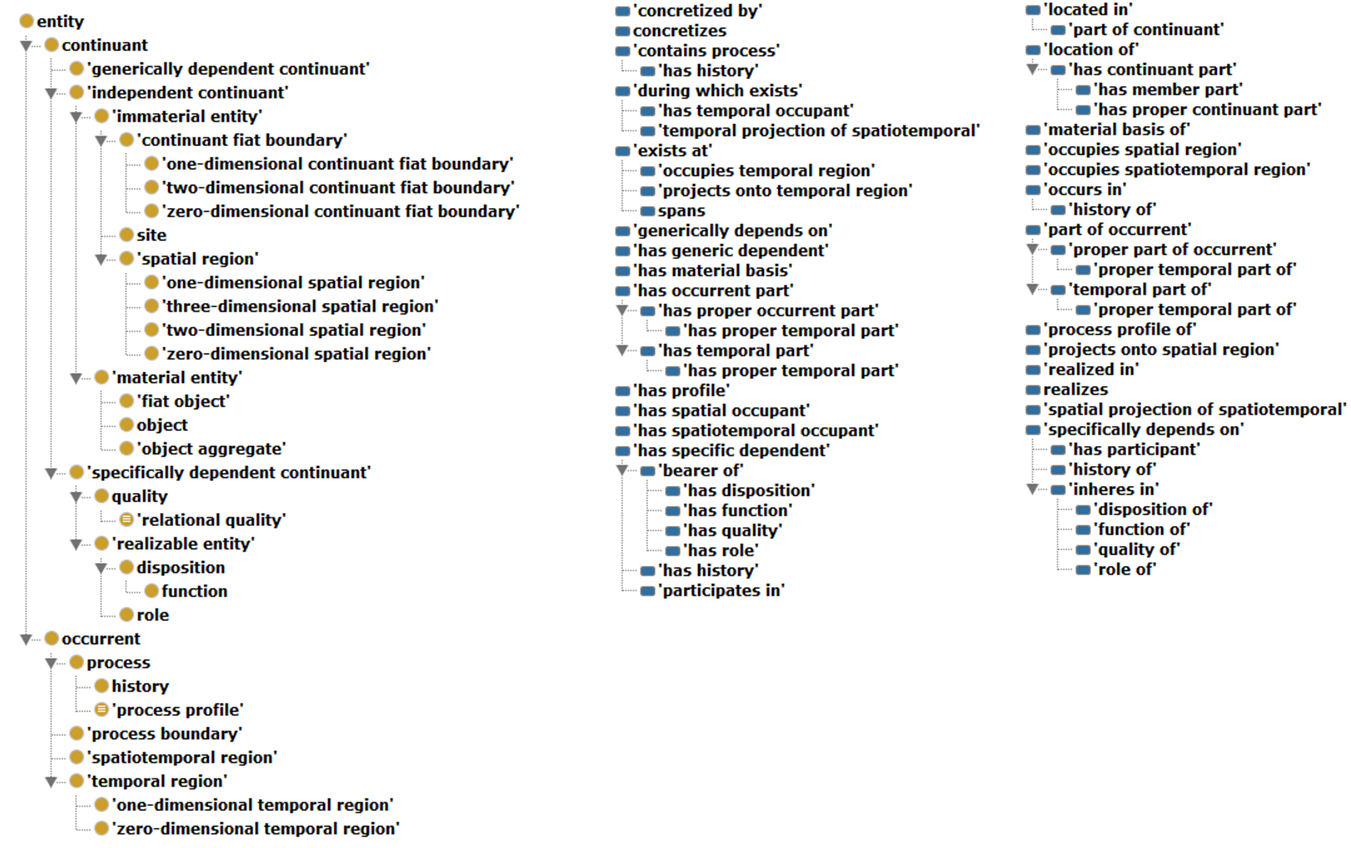
\includegraphics[width=120mm]{bfograph.png}
\caption{Classes and relations in BFO 2.0}
\label{fig:bfoclass}
\end{figure}

\newpage

\begin{figure}[h]
\centering
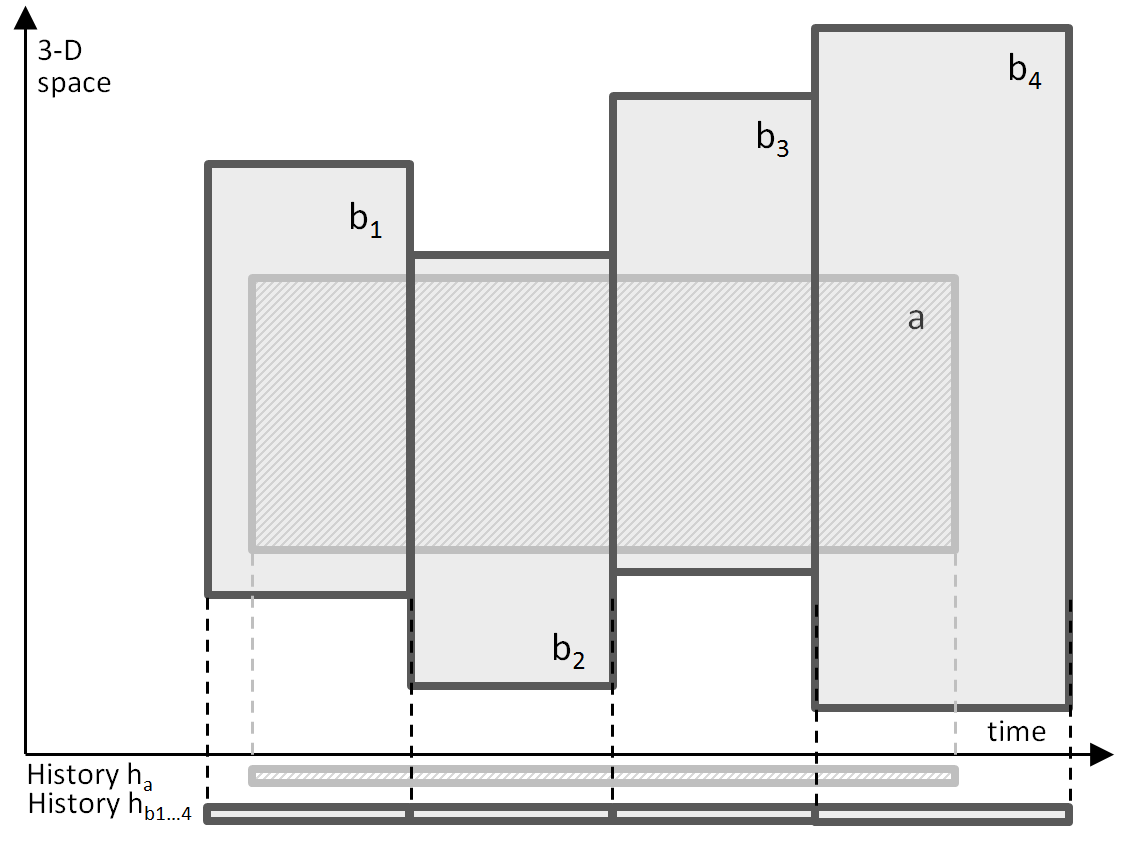
\includegraphics[width=120mm]{trgraph.png}
\caption{Permanent generic location as inclusion of histories. The object $a$ 
(depicted as a spatiotemporal ``worm'')is always included in some member of 
the class $B$, \emph{viz} $b_1$, $b_2$, $b_3$, $b_4$.}
\label{fig:trgraph}
\end{figure}


%%%%%%%%%%%%%%%%%%%%%%%%%%%%%%%%%%%
%%   %%
%% Tables    %%
%%   %%
%%%%%%%%%%%%%%%%%%%%%%%%%%%%%%%%%%%
\newpage
%% Use of \listoftables is discouraged.
%%
\section*{Tables}

\todo[inline, size=\tiny]{Big table, encompassing all examples and competency questions.
The source of this table is an Excel spreadsheet, from which a PDF file was created}   


Table 1. Results \\

examples and competency questions for both TR and TQC approaches. For each example and modelling 
approach the satisfiability is given: Y = satisfiable and N = not satisfiable. The reasoning 
example can be inspected in the additional files. 

 
\newpage


%%%%%%%%%%%%%%%%%%%%%%%%%%%%%%%%%%%
%%   %%
%% Additional Files  %%
%%   %%
%%%%%%%%%%%%%%%%%%%%%%%%%%%%%%%%%%%

\section*{Additional Files}
  
  
\subsection*{BFO OWL with temporalized relations}
This file (bfo\_tr.owl) corresponds to ``BFO OWL Graz'' as released in July 2012. It includes temporalized 
relations such as ``has continuant part at all times'', ``inheres in at some time'' etc.

\subsection*{BFO OWL with temporally qualified continuants}
This file (bfo\_tqc.owl)corresponds does not include temporalized relations and strictly follows the relations
as provided by the BFO reference guide. All ternary relations are reduced to binary object properties involving temporally qualified continuants (TQCs).
For the handling of TQCs additional object properties were added, as described in this paper. 

\subsection*{examples for temporalized relations}
This file (bfo\_tr\_uc.owl)contains the examples as described in this paper. 
It imports bfo\_tr.owl.

\subsection*{examples for temporally qualified continuants}
This file (bfo\_tqc\_uc.owl)contains the examples as described in this paper. 
It imports bfo\_tqc.owl.


\end{bmcformat}
\end{document}






